% Options for packages loaded elsewhere
\PassOptionsToPackage{unicode}{hyperref}
\PassOptionsToPackage{hyphens}{url}
%
\documentclass[
]{book}
\usepackage{lmodern}
\usepackage{amssymb,amsmath}
\usepackage{ifxetex,ifluatex}
\ifnum 0\ifxetex 1\fi\ifluatex 1\fi=0 % if pdftex
  \usepackage[T1]{fontenc}
  \usepackage[utf8]{inputenc}
  \usepackage{textcomp} % provide euro and other symbols
\else % if luatex or xetex
  \usepackage{unicode-math}
  \defaultfontfeatures{Scale=MatchLowercase}
  \defaultfontfeatures[\rmfamily]{Ligatures=TeX,Scale=1}
\fi
% Use upquote if available, for straight quotes in verbatim environments
\IfFileExists{upquote.sty}{\usepackage{upquote}}{}
\IfFileExists{microtype.sty}{% use microtype if available
  \usepackage[]{microtype}
  \UseMicrotypeSet[protrusion]{basicmath} % disable protrusion for tt fonts
}{}
\makeatletter
\@ifundefined{KOMAClassName}{% if non-KOMA class
  \IfFileExists{parskip.sty}{%
    \usepackage{parskip}
  }{% else
    \setlength{\parindent}{0pt}
    \setlength{\parskip}{6pt plus 2pt minus 1pt}}
}{% if KOMA class
  \KOMAoptions{parskip=half}}
\makeatother
\usepackage{xcolor}
\IfFileExists{xurl.sty}{\usepackage{xurl}}{} % add URL line breaks if available
\IfFileExists{bookmark.sty}{\usepackage{bookmark}}{\usepackage{hyperref}}
\hypersetup{
  pdftitle={Boletín Estadístico Sede La Paz},
  pdfauthor={ Universidad Nacional de Colombia   Sede La Paz},
  hidelinks,
  pdfcreator={LaTeX via pandoc}}
\urlstyle{same} % disable monospaced font for URLs
\usepackage{longtable,booktabs}
% Correct order of tables after \paragraph or \subparagraph
\usepackage{etoolbox}
\makeatletter
\patchcmd\longtable{\par}{\if@noskipsec\mbox{}\fi\par}{}{}
\makeatother
% Allow footnotes in longtable head/foot
\IfFileExists{footnotehyper.sty}{\usepackage{footnotehyper}}{\usepackage{footnote}}
\makesavenoteenv{longtable}
\usepackage{graphicx}
\makeatletter
\def\maxwidth{\ifdim\Gin@nat@width>\linewidth\linewidth\else\Gin@nat@width\fi}
\def\maxheight{\ifdim\Gin@nat@height>\textheight\textheight\else\Gin@nat@height\fi}
\makeatother
% Scale images if necessary, so that they will not overflow the page
% margins by default, and it is still possible to overwrite the defaults
% using explicit options in \includegraphics[width, height, ...]{}
\setkeys{Gin}{width=\maxwidth,height=\maxheight,keepaspectratio}
% Set default figure placement to htbp
\makeatletter
\def\fps@figure{htbp}
\makeatother
\setlength{\emergencystretch}{3em} % prevent overfull lines
\providecommand{\tightlist}{%
  \setlength{\itemsep}{0pt}\setlength{\parskip}{0pt}}
\setcounter{secnumdepth}{5}
\usepackage{booktabs}
\usepackage[]{natbib}
\bibliographystyle{apalike}

\title{Boletín Estadístico Sede La Paz}
\author{ Universidad Nacional de Colombia Sede La Paz}
\date{Última actualización: 05 de octubre de 2020}

\begin{document}
\maketitle

{
\setcounter{tocdepth}{1}
\tableofcontents
}
\hypertarget{portada}{%
\chapter*{Portada}\label{portada}}
\addcontentsline{toc}{chapter}{Portada}

\textbf{Comentarios, sugerencias e inquietudes}

\textbf{AAAA AAAA AAAA}
Cargo:
Email: \href{mailto:mail@unal.edu.co}{\nolinkurl{mail@unal.edu.co}}
Teléfono: (1) 3165000 extensión \_\_\_\_

\textbf{Sistema Estadístico UNAL}

El Boletín Estadísco de la Sede La Paz de la Universidad Nacional de Colombia hace parte integral del \emph{sistema estadístico institucional}. Para aquellos interesados en conocer la información estadística general de la Universidad así como de las demás sedes que hacen parte de esta institución, los invitamos a ingresar al sitio web de \href{http://estadisticas.unal.edu.co/home/}{estadísticas institucionales} y a conocer los porqués de este sitio expresados en el siguiente video institucional.

\hypertarget{Presenta}{%
\chapter*{Presentación}\label{Presenta}}
\addcontentsline{toc}{chapter}{Presentación}

\hypertarget{intro}{%
\chapter*{Introducción}\label{intro}}
\addcontentsline{toc}{chapter}{Introducción}

\hypertarget{mision}{%
\section*{Misión}\label{mision}}
\addcontentsline{toc}{section}{Misión}

Como Universidad de la nación fomenta el acceso con equidad al sistema educativo colombiano, provee la mayor oferta de programas académicos, forma profesionales competentes y socialmente responsables. Contribuye a la elaboración y resignificación del proyecto de nación, estudia y enriquece el patrimonio cultural, natural y ambiental del país. Como tal lo asesora en los órdenes científico, tecnológico, cultural y artístico con autonomía académica e investigativa.

\hypertarget{vision}{%
\section*{Visión 2034}\label{vision}}
\addcontentsline{toc}{section}{Visión 2034}

En el año 2034 somos la principal universidad colombiana, reconocida por su contribución a la Nación, y por su excelencia en los procesos de formación, investigación, e innovación social y tecnológica. Nuestra capacidad de reinventarnos nos ha llevado a tener una organización académica y administrativa novedosa, flexible, eficiente y sostenible, con comunicación transparente y efectiva en su interior, con la Nación y con el mundo, y comprometida con los procesos de transformación social requeridos para alcanzar una sociedad equitativa, incluyente y en paz.

\hypertarget{hist}{%
\section*{Historia}\label{hist}}
\addcontentsline{toc}{section}{Historia}

La sede De La Paz de la Universidad Nacional de Colombia fue creada mediante el \href{http://www.legal.unal.edu.co/rlunal/home/doc.jsp?d_i=89757}{Acuerdo 250} de 2017 del Consejo Superior Universitario CSU de la Universidad Nacional de Colombia. Mediante \href{http://www.legal.unal.edu.co/rlunal/home/doc.jsp?d_i=93599}{Acuerdo 301} de 2019 del CSU, se crea el Programa de Admisión Especial para los programas de pregrado de la Sede de La Paz de la Universidad Nacional de Colombia el cual se definió para ser implementado en un lapso de de tres años y aplicado a la zona de influencia que defina la Universidad (Artículo 1).

Para los periodos 2019-2 y 2020-1 la zona de influencia incluyó los aspirantes provenienets de los 25 municipios que conforman el Departamento Del Cesar. Para la convocatoria del periodo 2020-2, además de los aspirantes provenientes del Departamento del Cesar, se incluyeron los provenientes de los departamentos de Magdalena y La Guajira.

\hypertarget{ubica}{%
\section*{Ubicación}\label{ubica}}
\addcontentsline{toc}{section}{Ubicación}

La Sede La Paz de la Universidad Nacional de Colombia se encuentra ubicada en la Carretera Nacional kilómetro 9 Vía Valledupar - La Paz, Cesar-Colombia.

\hypertarget{paespaz}{%
\section*{Programa de Admisión Especial - La Paz}\label{paespaz}}
\addcontentsline{toc}{section}{Programa de Admisión Especial - La Paz}

Mediante \href{http://www.legal.unal.edu.co/rlunal/home/doc.jsp?d_i=93599}{Acuerdo 301} de 2019 del CSU, se crea el Programa de Admisión Especial para los programas de pregrado de la Sede de La Paz de la Universidad Nacional de Colombia el cual se definió para ser implementado en un lapso de de tres años y aplicado a la zona de influencia que defina la Universidad (Artículo 1).

Para los periodos 2019-2 y 2020-1 la zona de influencia incluyó los aspirantes provenienets de los 25 municipios que conforman el Departamento Del Cesar. Para la convocatoria del periodo 2020-2, además de los aspirantes provenientes del Departamento del Cesar, se incluyeron los provenientes de los departamentos de Magdalena y La Guajira.

\hypertarget{Prog}{%
\chapter{Programas Académicos}\label{Prog}}

\hypertarget{pregrado}{%
\section{Pregrado}\label{pregrado}}

\hypertarget{Aspirantes}{%
\chapter{Aspirantes y Admitidos}\label{Aspirantes}}

Este capítulo presenta el consolidado de las principales características asociadas a la información estadística oficial de los aspirantes y admitidos a pregrado en la sede La Paz de la Universidad Nacional de Colombia. A continuación, se presenta una breve descripción de las secciones que hacen parte de este capítulo así como la ubicación del sitio web en donde se presentan las definiciones, los estándares y las codificaciones/clasificaciones que hacen parte de la información acá contenida (\emph{metadatos}) y cuya exploración y lectura, sin duda, facilitará el entendimiento de las cifras asociadas a las poblaciones de aspirantes y admitidos en esta sede de la Universidad.

La Sede La Paz en la actualidad no cuenta con programas de postgrado. Por lo anterior, en este capítulo no se dispone información estadística para este nivel de formación.

\textbf{Secciones}

El proceso de formación en pregrado en la Sede La Paz se da a la luz de los lineamientos definidos en el Programa Especial de Admisión creado mediante el \href{http://www.legal.unal.edu.co/rlunal/home/doc.jsp?d_i=93599}{Acuerdo 301} de 2019 del CSU.

\begin{itemize}
\item
  \protect\hyperlink{AspPre}{Aspirantes a pregrado}: contiene la información oficial del total de aspirantes a pregrado en la Sede La Paz de la Universidad Nacional de Colombia y que se incribieron a través del Programa Especial de esta sede creado mediante el \href{http://www.legal.unal.edu.co/rlunal/home/doc.jsp?d_i=93599}{Acuerdo 301} de 2019 del CSU.
\item
  \protect\hyperlink{AdmPre}{Admitidos a pregrado}: contiene la información oficial del total de admitidos a pregrado en la Sede La Paz de la Universidad Nacional de Colombia y que se incribieron a través del Programa Especial de Admisión creado mediante el \href{http://www.legal.unal.edu.co/rlunal/home/doc.jsp?d_i=93599}{Acuerdo 301} de 2019 del CSU.
\end{itemize}

\textbf{Metadatos}

La construcción de las cifras oficiales de aspirantes y admitidos a pregrado en la Sede La Paz, las definiciones que hacen parte de estas así como las codificaciones y clasificaciones aquí empleadas se encuentran contenidas en la sección \textbf{Aspirantes y Admitidos} del capítulo de \emph{Metadatos} de las cifras oficiales generales que hacen parte de la página de \href{http://estadisticas.unal.edu.co/home/}{estadísticas} de la Universidad Nacional de Colombia. Invitamos a los lectores a explorar y conocer estos metadatos los cuales, además de orientar y facilitar el entendimiento de la información acá expuesta, se encuentran disponibles en el siguiente enlace.

\begin{itemize}
\tightlist
\item
  \href{http://estadisticas.unal.edu.co/menu-principal/cifras-generales/metadatos/cifras-generales/}{Metadatos Cifras Oficiales Universidad Nacional de Colombia}
\end{itemize}

\hypertarget{AspPre}{%
\section{Aspirantes a pregrado}\label{AspPre}}

A continuación, se presentan las principales características asociadas a los aspirantes a pregrado de la \textbf{Sede La Paz} de la Universidad Nacional de Colombia. En específico, se presenta la evolución histórica de los aspirantes a pregrado desde diferentes perspectivas: general, sexo, grupos de edad, estrato socioeconómico, tasa de absorción y departamentos y municipios de residencia de los mismos. Para cada una de las variables analizadas se presenta la evolución histórica (\emph{serie de tiempo}) así como el comportamiento actual (\emph{estado actual}) derivado de las últimas mediciones disponibles.

\hypertarget{evoluciuxf3n-histuxf3rica}{%
\subsection{Evolución Histórica}\label{evoluciuxf3n-histuxf3rica}}

A continuación, la Figura \ref{fig:F1AspPre}, presenta la evolución histórica -\emph{desde el periodo 20192}-, del total de aspirantes a pregrado en la sede.

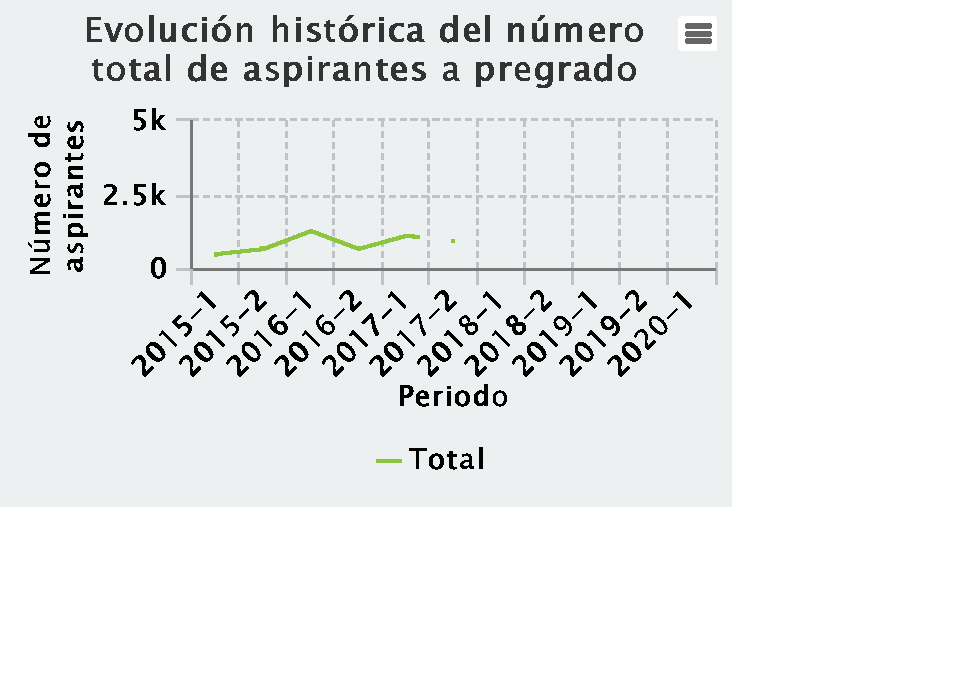
\includegraphics{BoletinLaPaz_files/figure-latex/F1AspPre-1.pdf}

\hypertarget{informaciuxf3n-por-sexo}{%
\subsection{Información por sexo}\label{informaciuxf3n-por-sexo}}

A continuación, las figuras \ref{fig:F2AspPre} y \ref{fig:F3AspPre} presentan, respectivamente, la evolución histórica y el comportamiento actual del total de aspirantes a pregrado según el sexo biológico.

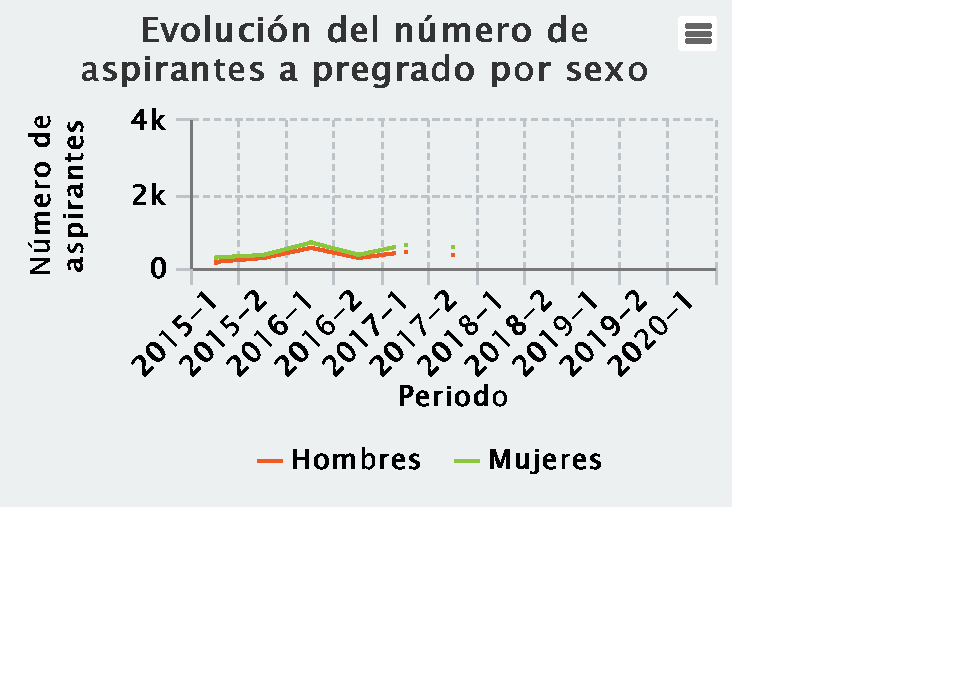
\includegraphics{BoletinLaPaz_files/figure-latex/F2AspPre-1.pdf}
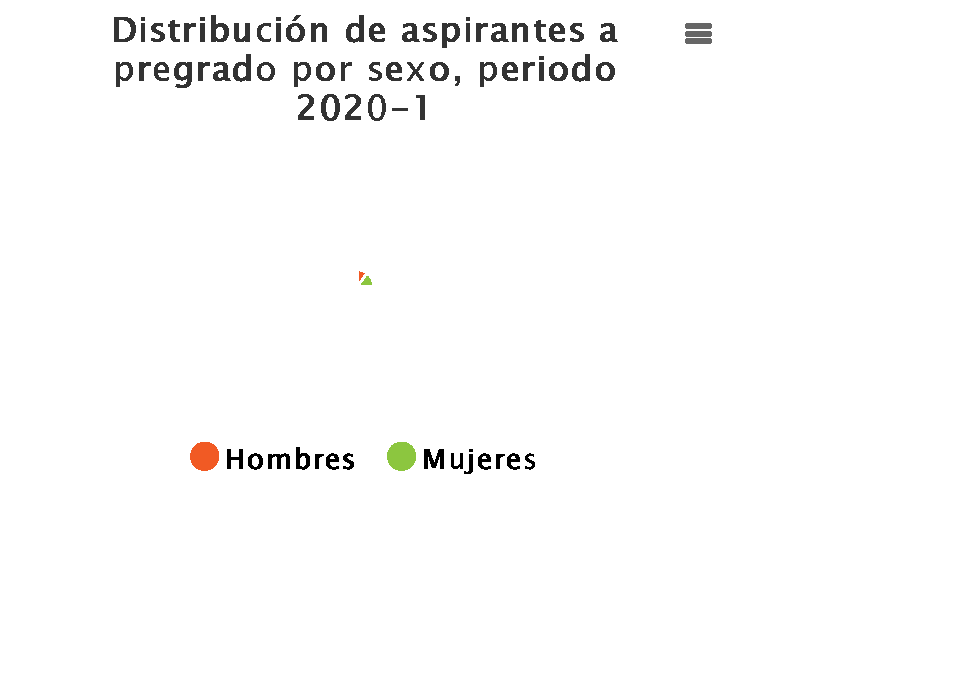
\includegraphics{BoletinLaPaz_files/figure-latex/F3AspPre-1.pdf}

\hypertarget{informaciuxf3n-por-edad}{%
\subsection{Información por edad}\label{informaciuxf3n-por-edad}}

A continuación, las figuras \ref{fig:F4AspPre} y \ref{fig:F5AspPre} presentan, respectivamente, la evolución histórica y el comportamiento actual del total de aspirantes a pregrado por grupos de edad.

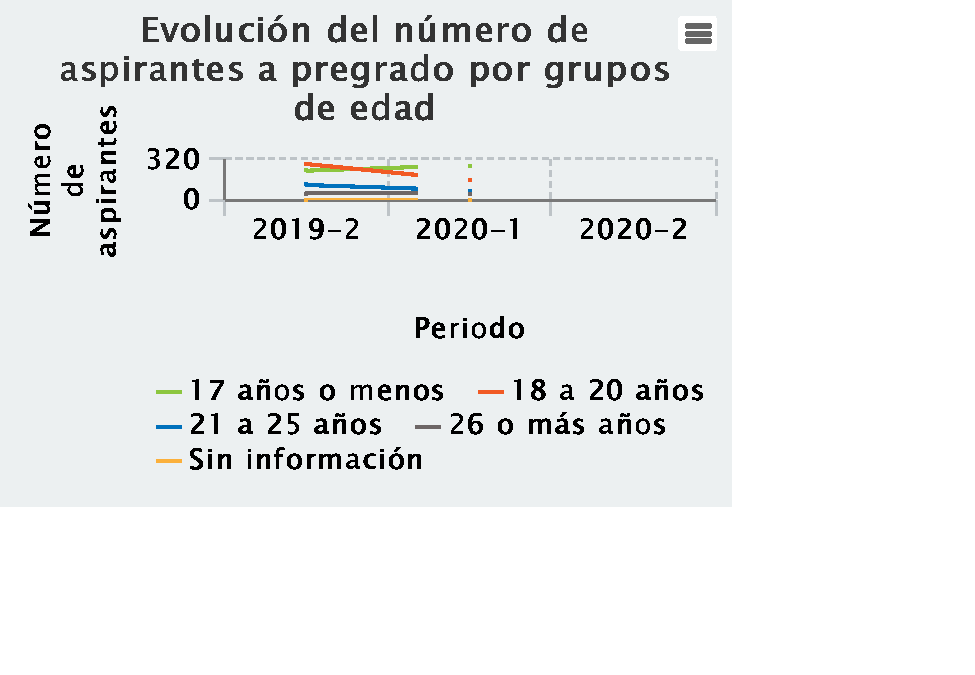
\includegraphics{BoletinLaPaz_files/figure-latex/F4AspPre-1.pdf}
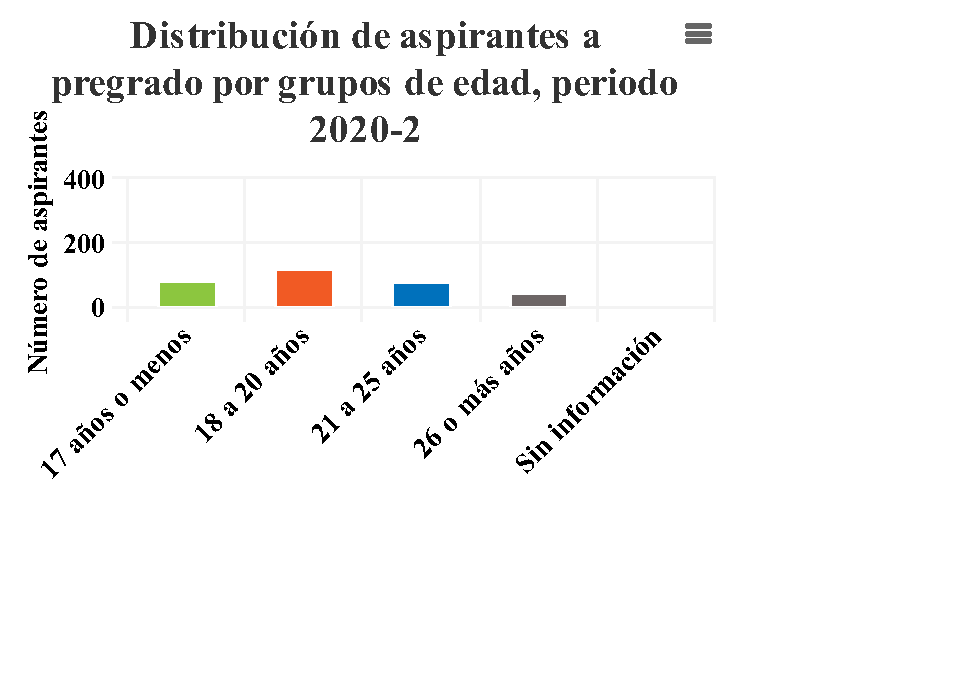
\includegraphics{BoletinLaPaz_files/figure-latex/F5AspPre-1.pdf}

\hypertarget{informaciuxf3n-por-estrato-socioeconuxf3mico}{%
\subsection{Información por estrato socioeconómico}\label{informaciuxf3n-por-estrato-socioeconuxf3mico}}

A continuación, las figuras \ref{fig:F6AspPre} y \ref{fig:F7AspPre} presentan, respectivamente, la evolución histórica y el comportamiento actual del total de aspirantes a pregrado según el estrato socioeconómico de las viviendas en donde estos residen.

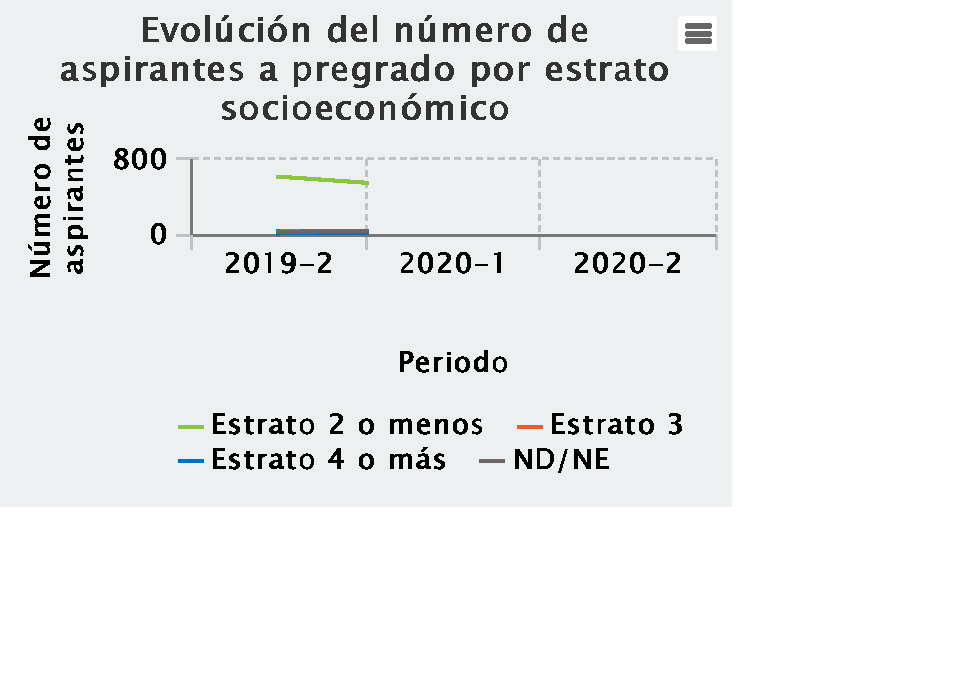
\includegraphics{BoletinLaPaz_files/figure-latex/F6AspPre-1.pdf}
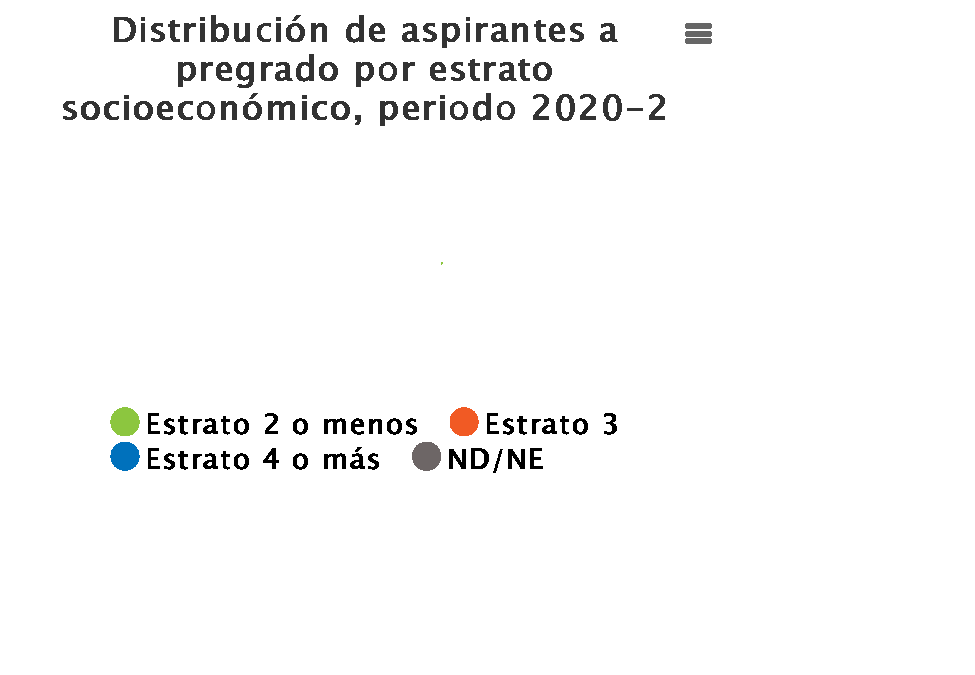
\includegraphics{BoletinLaPaz_files/figure-latex/F7AspPre-1.pdf}

\hypertarget{tasa-de-absorciuxf3n}{%
\subsection{Tasa de absorción}\label{tasa-de-absorciuxf3n}}

A continuación, las figuras \ref{fig:F8AspPre} y \ref{fig:F9AspPre} presentan, respectivamente, la evolución histórica y el comportamiento actual del total de aspirantes admitidos a pregrado en la Sede La Paz de la Universidad Nacional de Colombia.

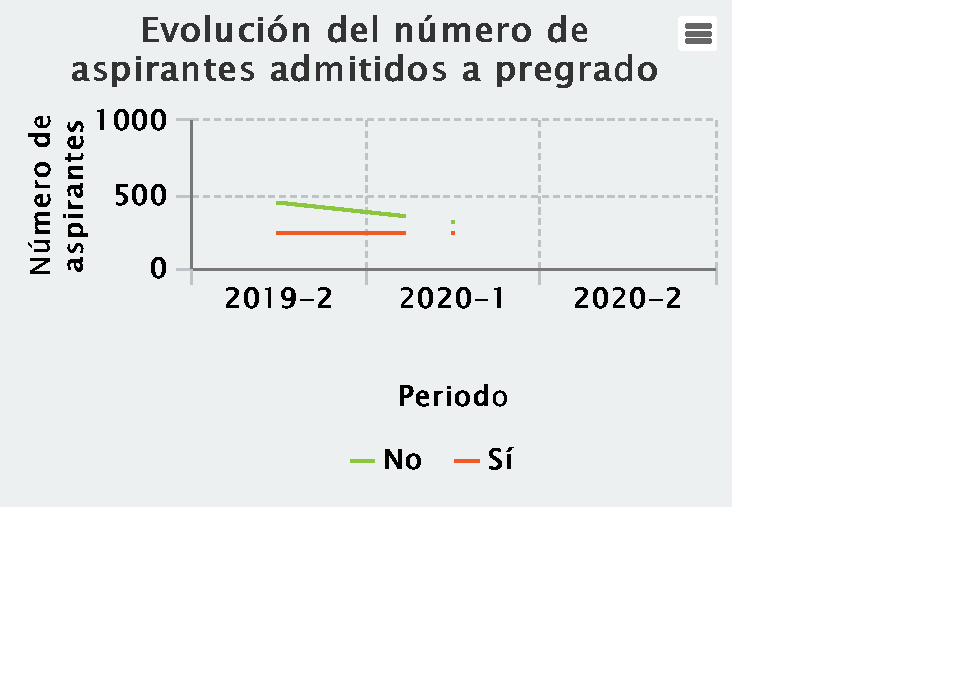
\includegraphics{BoletinLaPaz_files/figure-latex/F8AspPre-1.pdf}
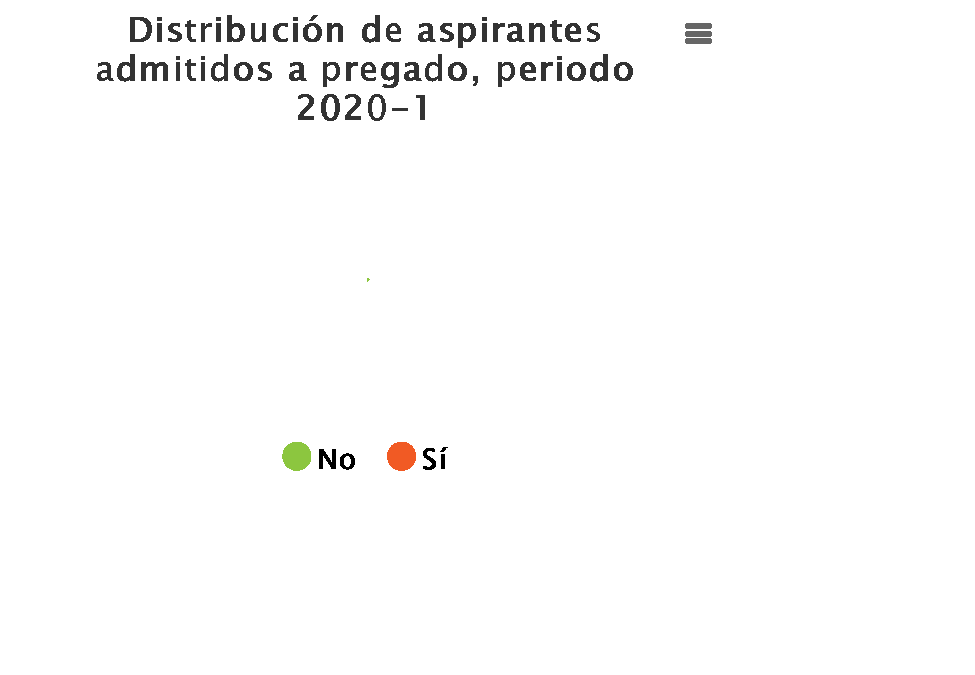
\includegraphics{BoletinLaPaz_files/figure-latex/F9AspPre-1.pdf}

\hypertarget{tablas-cifras-agregadas}{%
\subsection{Tablas cifras agregadas}\label{tablas-cifras-agregadas}}

A continuación se presentan, a través de tablas, los agregados/consolidados históricos del total de aspirantes a pregrado de la Sede La Paz por departamentos y municipios de procedencia.

Los interesados en \emph{imprimir}, \emph{copiar} o \emph{descargar} estas cifras, pueden hacerlo a través de las múltiples opciones que se ofrecen en la parte superior izquierda de cada una de las tablas que se presentan a continuación (Copiar, CSV, Excel, PDF e Imprimir). Así mismo estas tablas, dada su naturaleza web, permiten filtrar los resultados por aquellas variables de interés.

\hypertarget{departamentos-y-municipios-de-procedencia}{%
\subsubsection{Departamentos y municipios de procedencia}\label{departamentos-y-municipios-de-procedencia}}

A continuación, la tabla \ref{fig:F10AspPre} presenta el acumulado \textbf{histórico}, por \textbf{años y semestres}, de los aspirantes a pregrado por departamentos y municipios de procedencia en la Sede La Paz.

\begin{figure}
\centering
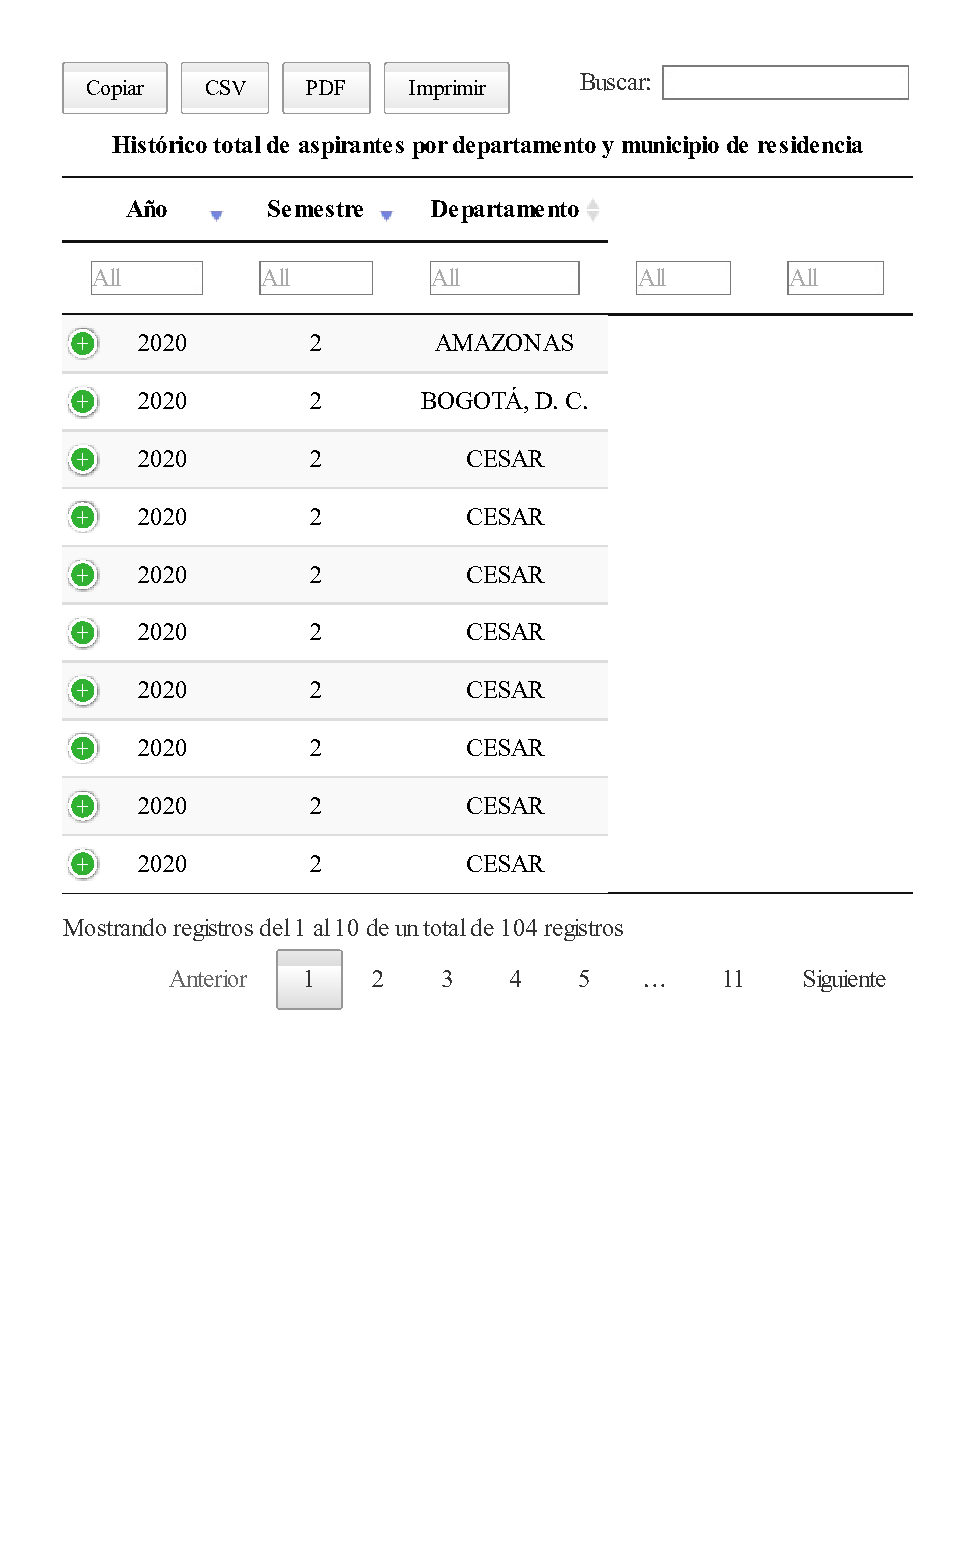
\includegraphics{BoletinLaPaz_files/figure-latex/F10AspPre-1.pdf}
\caption{\label{fig:F10AspPre}Fuente: Dirección Nacional de Planeación y Estadística con base en información de la Dirección Nacional de Admisiones}
\end{figure}

\hypertarget{AdmPre}{%
\section{Admitidos a pregrado}\label{AdmPre}}

A continuación, se presentan las principales características asociadas a los admitidos a pregrado de la Sede La Paz de la Universidad Nacional de Colombia. En específico, se presenta la evolución histórica de los admitidos a pregrado desde diferentes perspectivas: general, sexo, grupos de edad, estrato socioeconómico, departamentos y municipios de residencia así como los programas académicos, las facultades y las sedes andinas en las que estos se encuentran ubicados. Para cada una de las variables analizadas se presenta la evolución histórica (\emph{serie de tiempo}) así como el comportamiento actual (\emph{estado actual}) derivado de las últimas mediciones disponibles.

\hypertarget{evoluciuxf3n-histuxf3rica-1}{%
\subsection{Evolución Histórica}\label{evoluciuxf3n-histuxf3rica-1}}

A continuación, la Figura \ref{fig:F1AdmPre}, presenta la evolución histórica -\emph{desde el periodo 20192}-, del total de admitidos a pregrado en la sede.

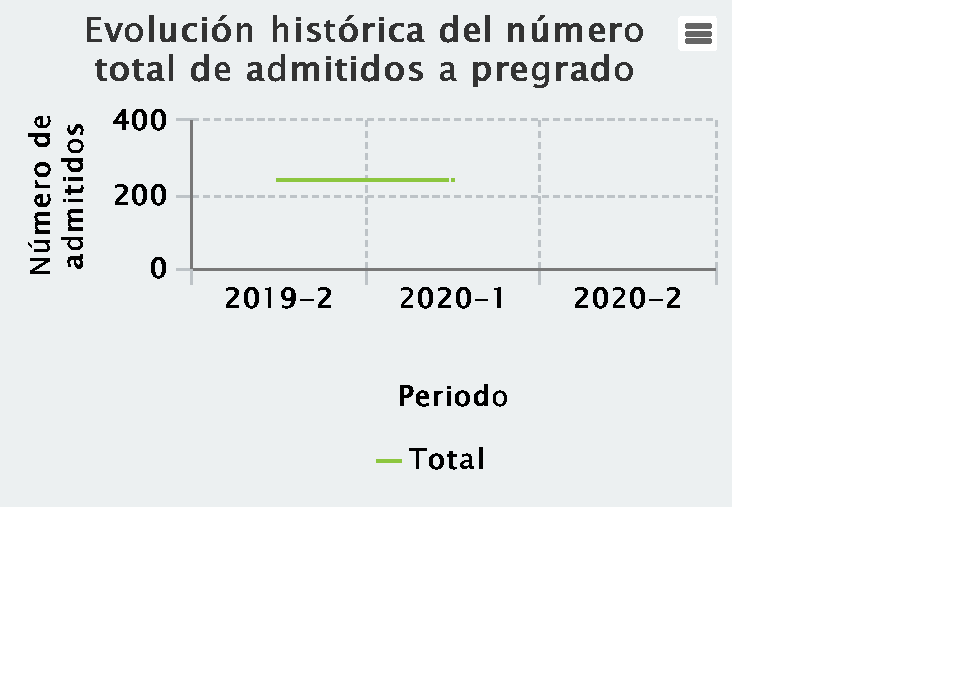
\includegraphics{BoletinLaPaz_files/figure-latex/F1AdmPre-1.pdf}

\hypertarget{informaciuxf3n-por-sexo-1}{%
\subsection{Información por sexo}\label{informaciuxf3n-por-sexo-1}}

A continuación, las figuras \ref{fig:F2AdmPre} y \ref{fig:F3AdmPre} presentan, respectivamente, la evolución histórica y el comportamiento actual del total de admitidos a pregrado según el sexo biológico.

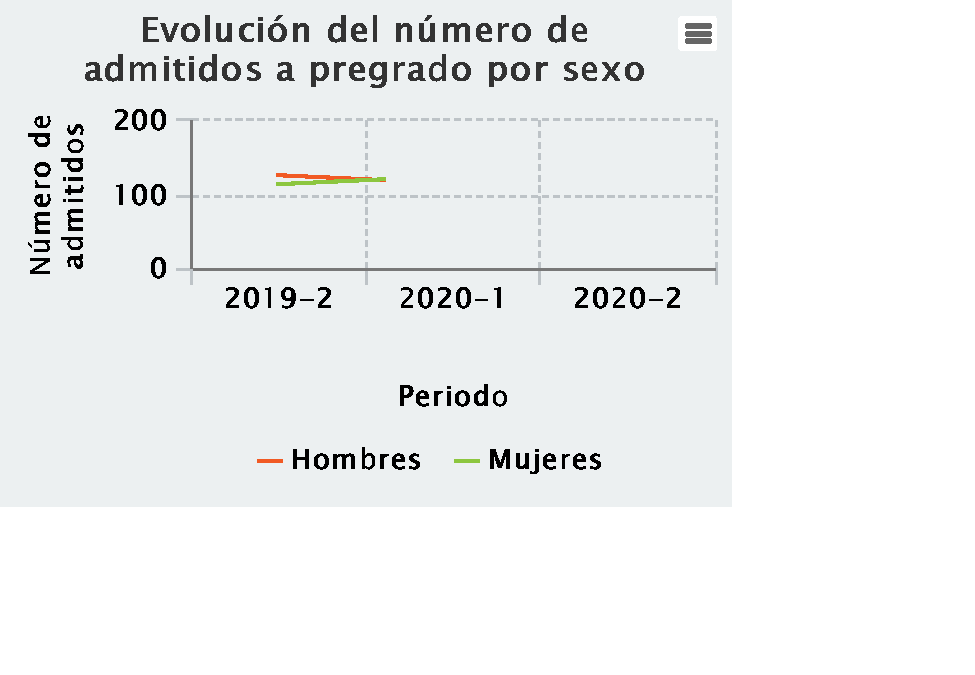
\includegraphics{BoletinLaPaz_files/figure-latex/F2AdmPre-1.pdf}
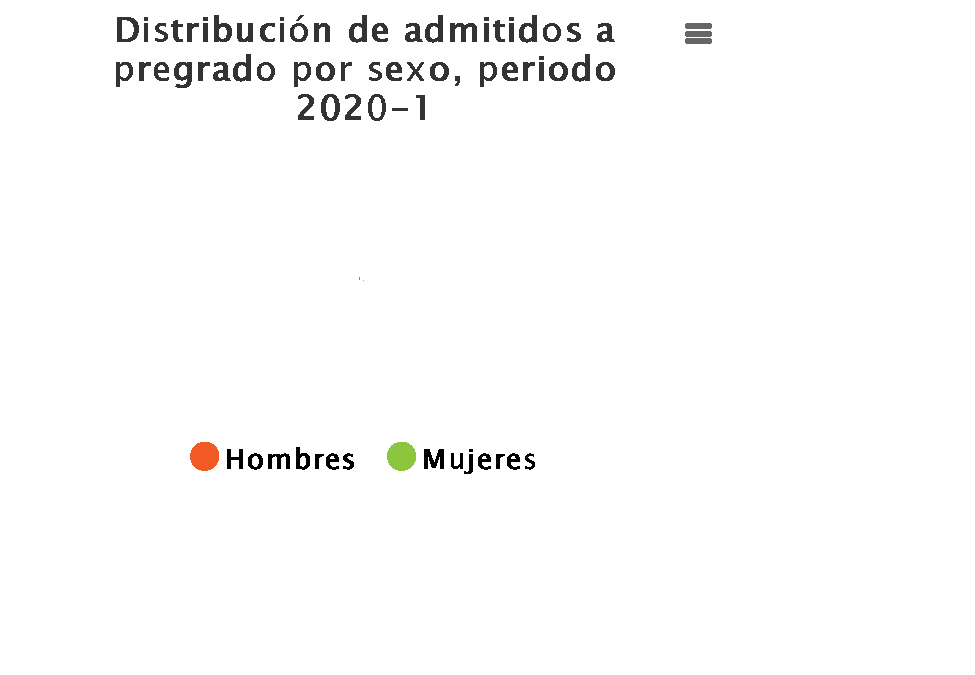
\includegraphics{BoletinLaPaz_files/figure-latex/F3AdmPre-1.pdf}

\hypertarget{informaciuxf3n-por-edad-1}{%
\subsection{Información por edad}\label{informaciuxf3n-por-edad-1}}

A continuación, las figuras \ref{fig:F4AdmPre} y \ref{fig:F5AdmPre} presentan, respectivamente, la evolución histórica y el comportamiento actual del total de admitidos a pregrado por grupos de edad.

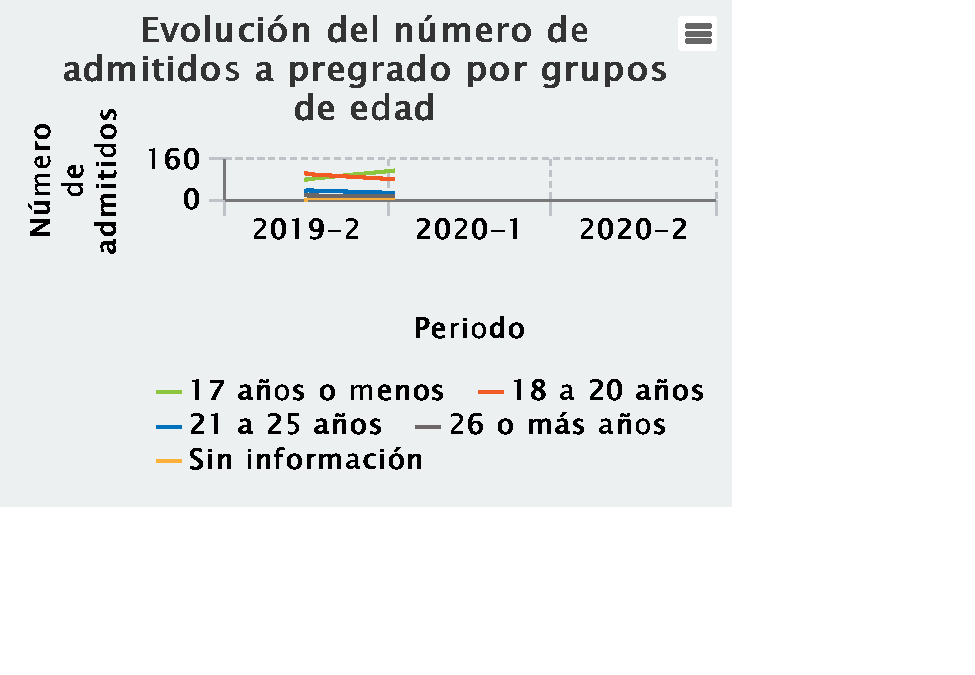
\includegraphics{BoletinLaPaz_files/figure-latex/F4AdmPre-1.pdf}
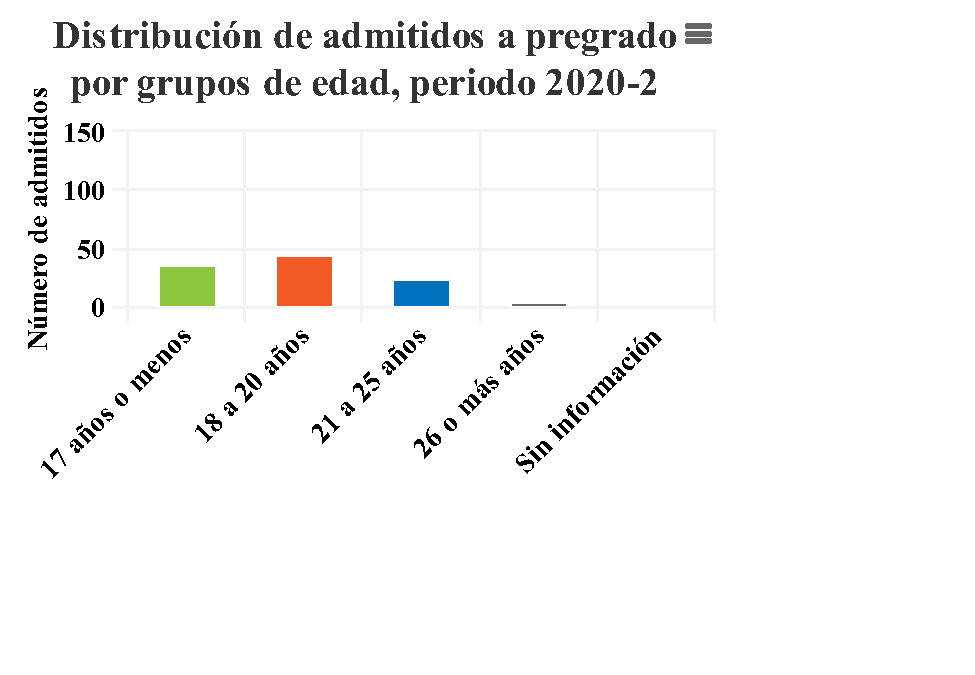
\includegraphics{BoletinLaPaz_files/figure-latex/F5AdmPre-1.pdf}

\hypertarget{informaciuxf3n-por-estrato-socioeconuxf3mico-1}{%
\subsection{Información por estrato socioeconómico}\label{informaciuxf3n-por-estrato-socioeconuxf3mico-1}}

A continuación, las figuras \ref{fig:F6AdmPre} y \ref{fig:F7AdmPre} presentan, respectivamente, la evolución histórica y el comportamiento actual del total de admitidos a pregrado según el estrato socioeconómico de las viviendas en donde estos residen.

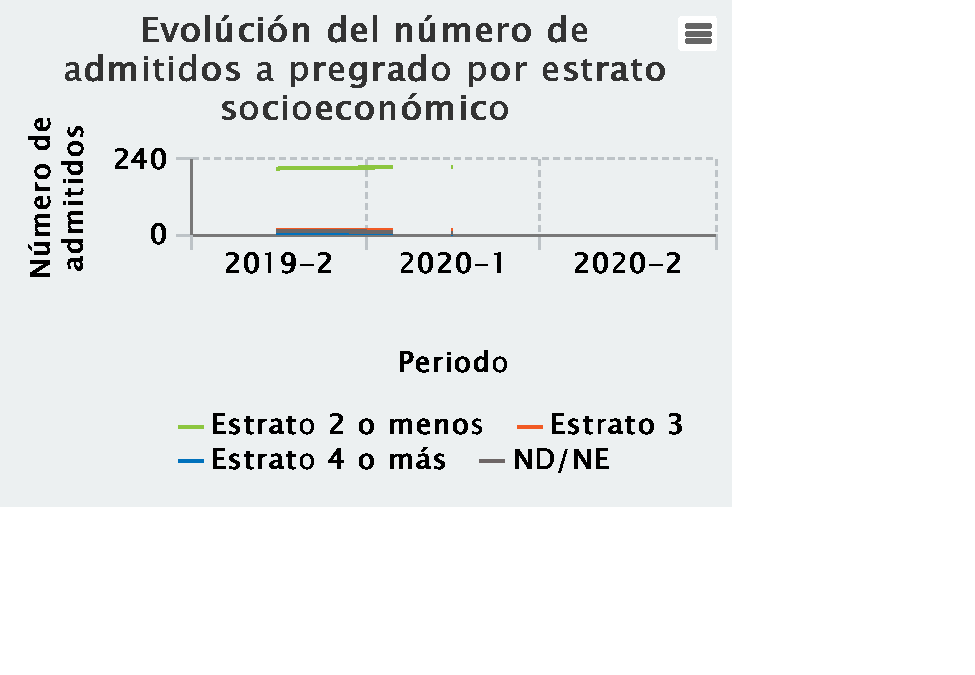
\includegraphics{BoletinLaPaz_files/figure-latex/F6AdmPre-1.pdf}
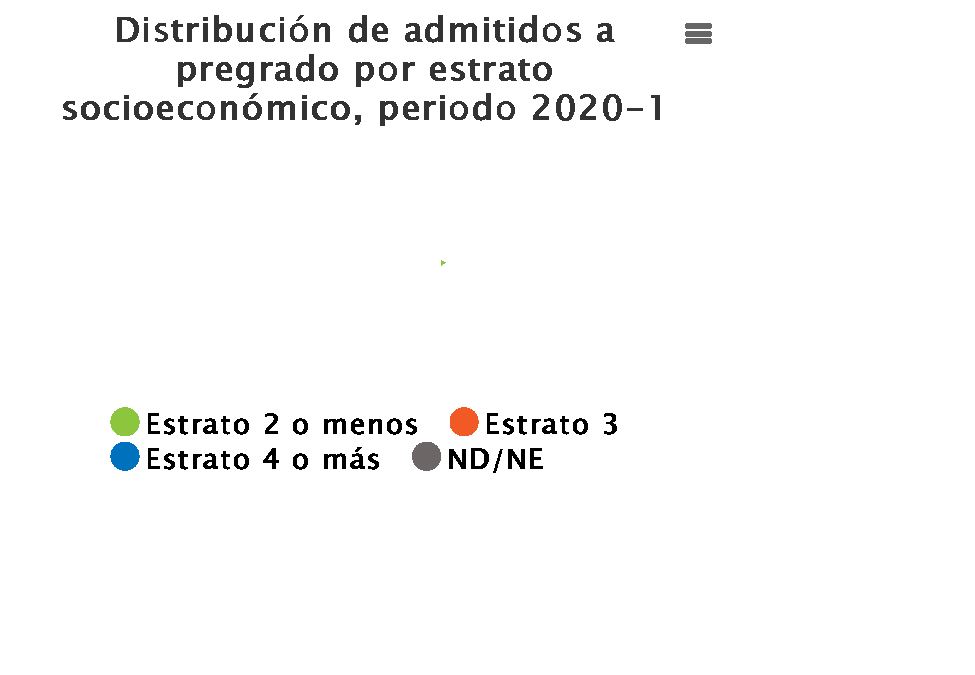
\includegraphics{BoletinLaPaz_files/figure-latex/F7AdmPre-1.pdf}

\hypertarget{tablas-cifras-agregadas-1}{%
\subsection{Tablas cifras agregadas}\label{tablas-cifras-agregadas-1}}

A continuación se presentan, a través de tablas, los agregados/consolidados históricos del total de admitidos a pregrado de la Sede La Paz por departamentos y municipios de procedencia, así como los programas académicos y las sedes andinas a las que estos pertecenecen.

Los interesados en \emph{imprimir}, \emph{copiar} o \emph{descargar} estas cifras, pueden hacerlo a través de las múltiples opciones que se ofrecen en la parte superior izquierda de cada una de las tablas que se presentan a continuación (Copiar, CSV, Excel, PDF e Imprimir). Así mismo estas tablas, dada su naturaleza web, permiten filtrar los resultados por aquellas variables de interés.

\hypertarget{departamentos-y-municipios-de-procedencia.}{%
\subsubsection{Departamentos y municipios de procedencia.}\label{departamentos-y-municipios-de-procedencia.}}

A continuación, la tabla \ref{fig:F8AdmPre} presenta el acumulado \textbf{histórico}, por \textbf{años y semestres}, en la Sede La Paz de los admitidos a pregrado por departamentos y municipios de procedencia.

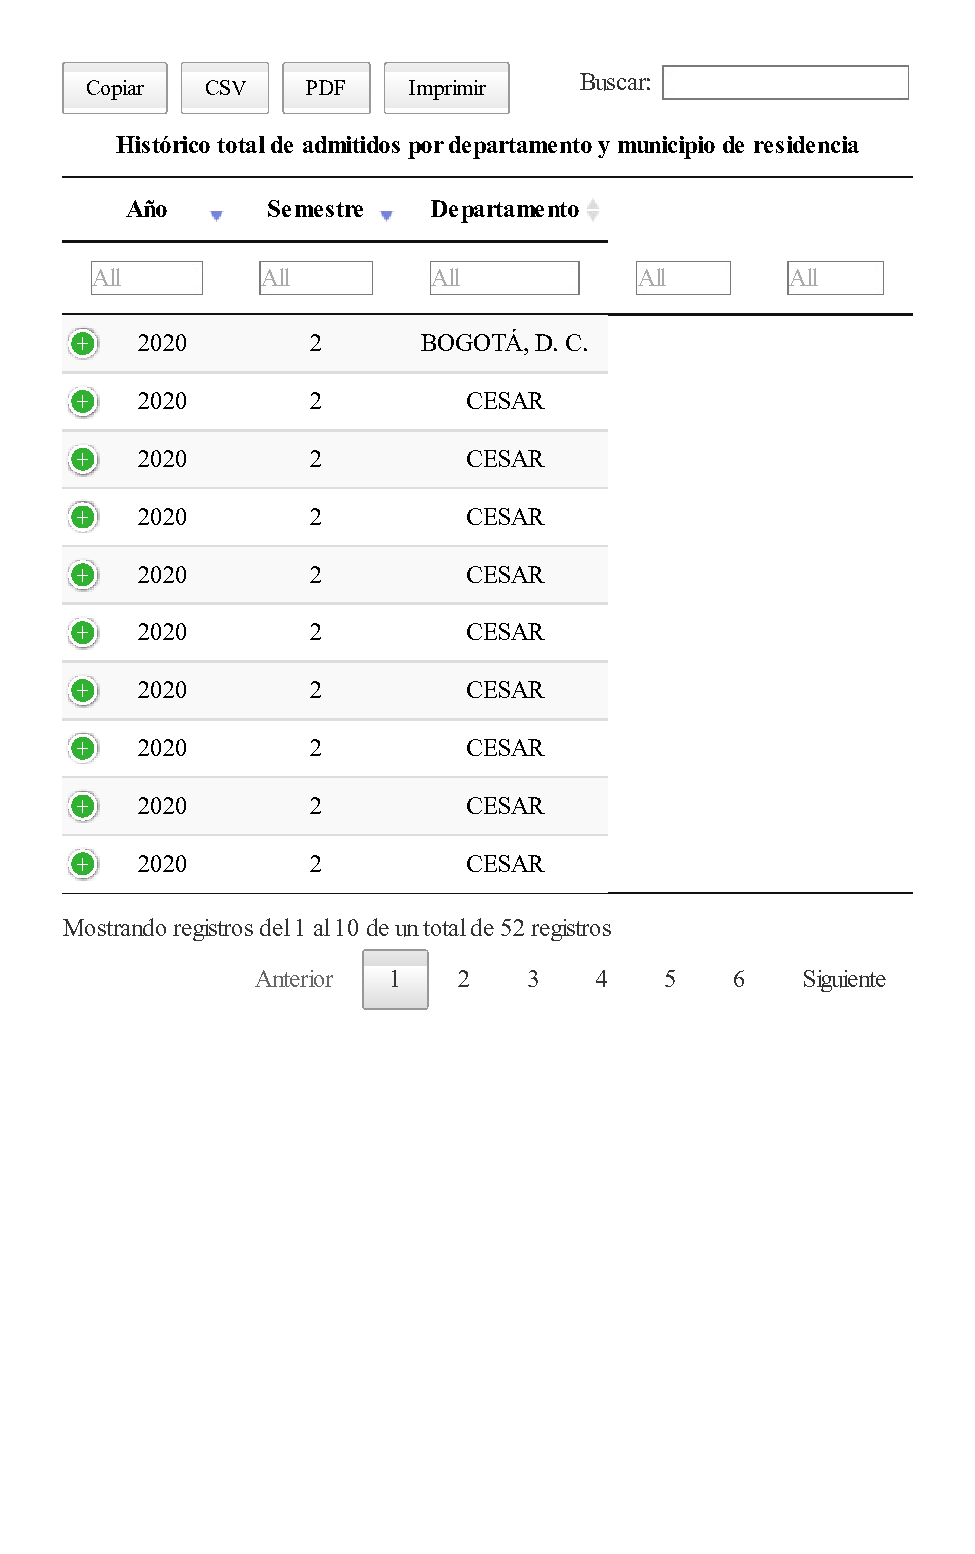
\includegraphics{BoletinLaPaz_files/figure-latex/F8AdmPre-1.pdf}

\hypertarget{programas-acaduxe9micos-de-pregrado}{%
\subsubsection{Programas académicos de pregrado}\label{programas-acaduxe9micos-de-pregrado}}

A continuación, la tabla \ref{fig:F9AdmPre} presenta el acumulado \textbf{histórico}, por \textbf{años y semestres}, en la Sede La Paz de los admitidos a pregrado por programas académicos y sedes andinas en las que estos se encuentran adscritos.

\begin{figure}
\centering
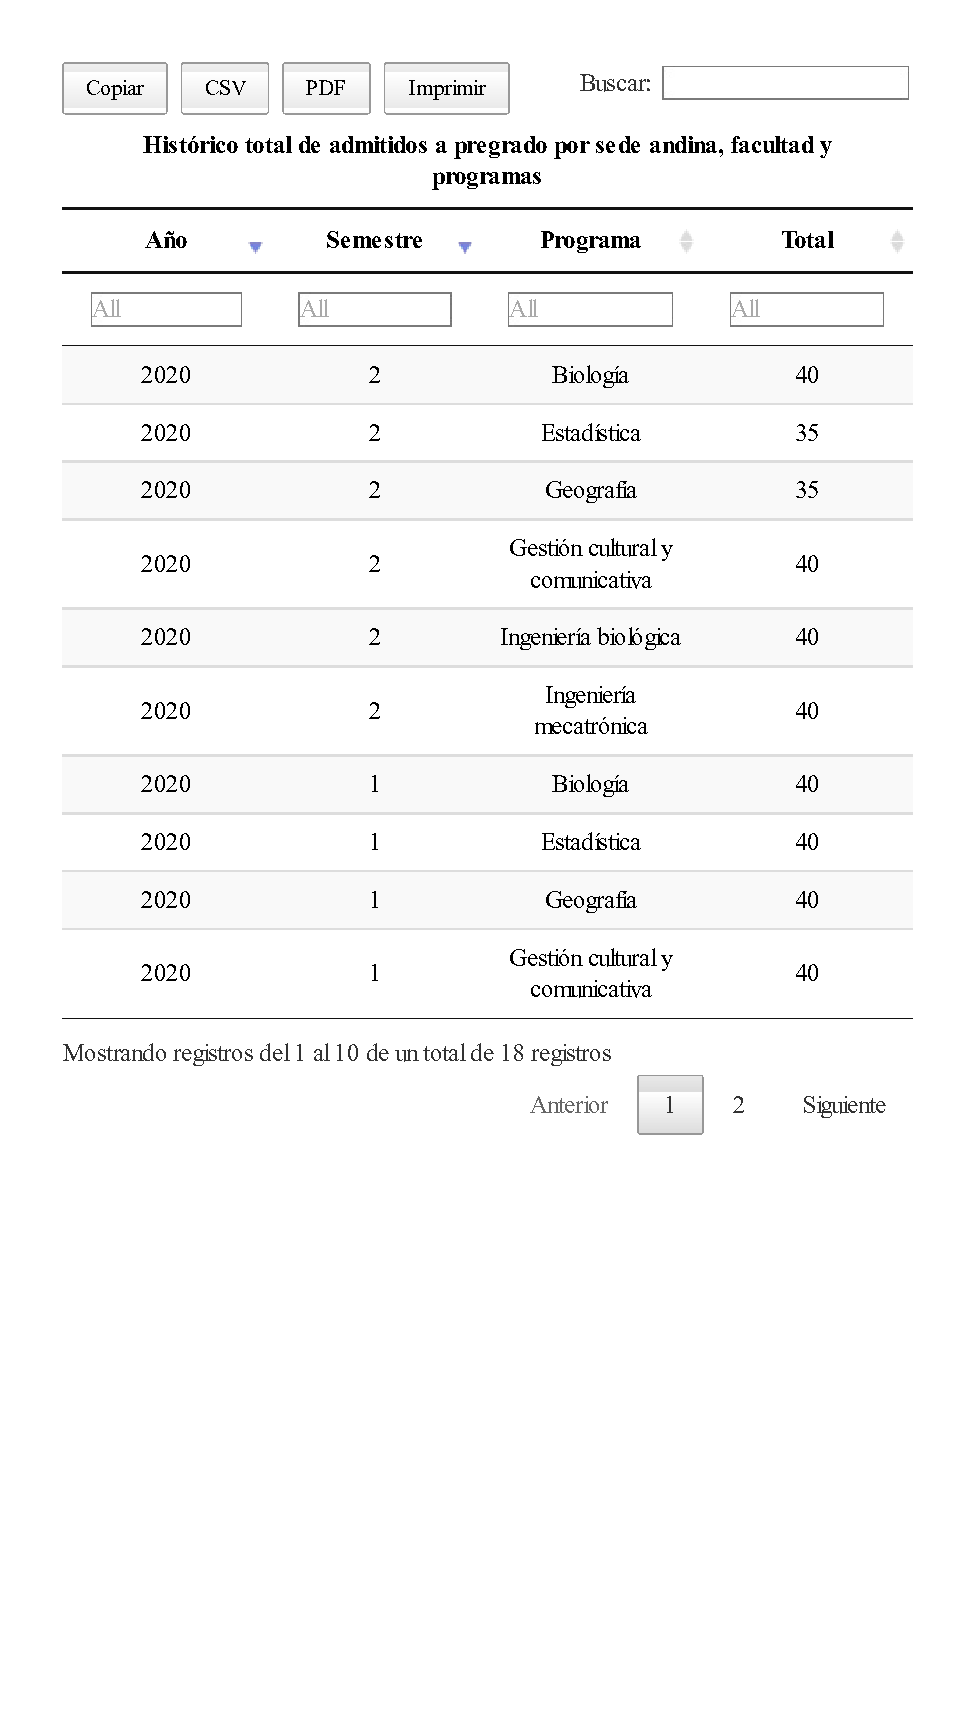
\includegraphics{BoletinLaPaz_files/figure-latex/F9AdmPre-1.pdf}
\caption{\label{fig:F9AdmPre}Fuente: Dirección Nacional de Planeación y Estadística con base en información de la Dirección Nacional de Admisiones}
\end{figure}

\hypertarget{Estudiantes}{%
\chapter{Estudiantes}\label{Estudiantes}}

Este capítulo presenta el consolidado de las principales características asociadas a la información estadística oficial de los estudiantes matriculados en pregrado en la sede La Paz de la Universidad Nacional de Colombia. A continuación, se presenta una breve descripción de las secciones que hacen parte de este capítulo así como la ubicación del sitio web en donde se presentan las definiciones, los estándares y las codificaciones/clasificaciones que hacen parte de la información acá contenida (\emph{metadatos}) y cuya exploración y lectura, sin duda, facilitará el entendimiento de las cifras asociadas a las poblaciones de estudiantes matriculados.

La Sede La Paz en la actualidad no cuenta con programas de postgrado. Por lo anterior, en este capítulo no se dispone información estadística para este nivel de formación.

\textbf{Secciones}

El proceso de formación en pregrado en la Sede La Paz se da a la luz de los lineamientos definidos en el Programa Especial de Admisión de esta sede creado mediante el \href{http://www.legal.unal.edu.co/rlunal/home/doc.jsp?d_i=93599}{Acuerdo 301} de 2019 del CSU. Teniendo en cuenta lo anterior, en este capítulo se presentan las estadísticas oficiales asociadas a la población de estudiantes matriculados en pregrado en la Sede La Paz de la Universidad Nacional de Colombia.

\begin{itemize}
\tightlist
\item
  \protect\hyperlink{MatPre}{Matriculados en pregrado}: contiene la información oficial del total de estudiantes matricualdos en pregrado en la Universidad y que han sido admitidos a través de la Sede La Paz.
\end{itemize}

\textbf{Metadatos}

La construcción de las cifras oficiales de estudiantes matriculados en pregrado de la Sede La Paz, las definiciones que hacen parte de estas así como las codificaciones y clasificaciones aquí empleadas se encuentran contenidas en la sección \textbf{Matriculados} del capítulo de \emph{Metadatos} de las cifras oficiales generales que hacen parte de la página de \href{http://estadisticas.unal.edu.co/home/}{estadísticas} de la Universidad Nacional de Colombia. Invitamos a los lectores a explorar y conocer estos metadatos los cuales, además de orientar y facilitar el entendimiento de la información acá expuesta, se encuentran disponibles en el siguiente enlace.

\begin{itemize}
\tightlist
\item
  \href{http://estadisticas.unal.edu.co/menu-principal/cifras-generales/metadatos/cifras-generales/}{Metadatos Cifras Oficiales Universidad Nacional de Colombia}
\end{itemize}

\hypertarget{MatPre}{%
\section{Matriculados en pregrado}\label{MatPre}}

A continuación, se presenta la información oficial del total de estudiantes matricualdos en pregrado en la Universidad y que han sido admitidos a través de la \textbf{Sede La Paz}. En específico, se presenta la evolución histórica de los matriculados en pregrado desde diferentes perspectivas: general, etapa de formación, sedes andinas, sexo, grupos de edad, estrato socioeconómico, departamentos y municipios de residencia y programas académicos en los que estos se encuentran matriculados. Para cada una de las variables analizadas se presenta la evolución histórica (\emph{serie de tiempo}) así como el comportamiento actual (\emph{estado actual}) derivado de las últimas mediciones disponibles.

\hypertarget{evoluciuxf3n-histuxf3rica-2}{%
\subsection{Evolución histórica}\label{evoluciuxf3n-histuxf3rica-2}}

A continuación, la Figura \ref{fig:F1MatPre}, presenta la evolución histórica -\emph{desde el periodo 20192}-, del total de matriculados en pregrado en la \textbf{Sede La Paz}.

\begin{figure}
\centering
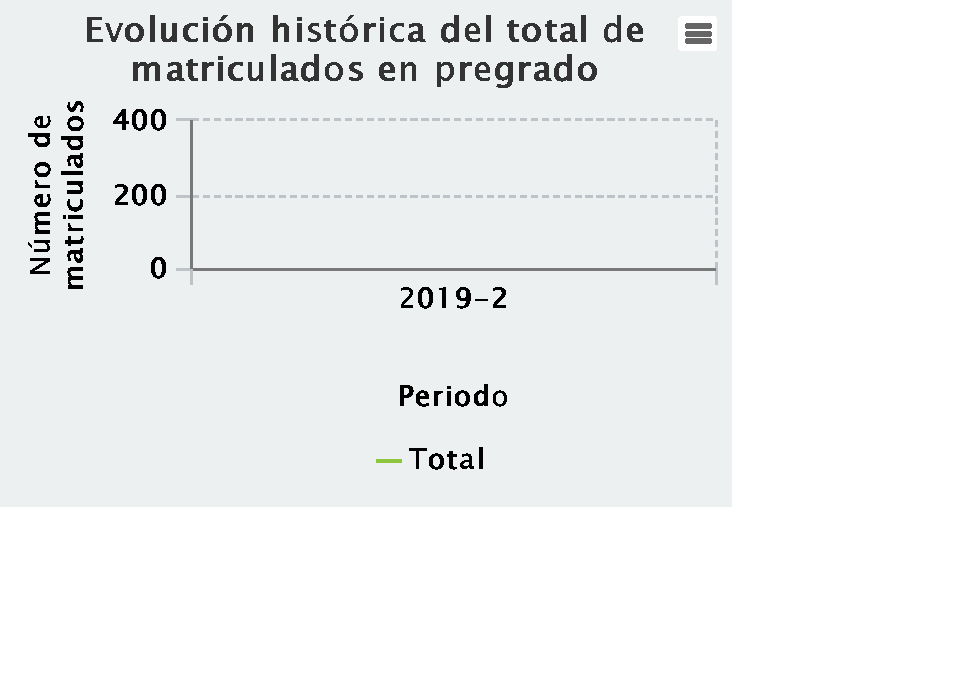
\includegraphics{BoletinLaPaz_files/figure-latex/F1MatPre-1.pdf}
\caption{\label{fig:F1MatPre}Fuente: Dirección Nacional de Planeación y Estadística con base en información de la Dirección Nacional Información Académica}
\end{figure}

\hypertarget{informaciuxf3n-por-sexo-2}{%
\subsection{Información por sexo}\label{informaciuxf3n-por-sexo-2}}

A continuación, las figuras \ref{fig:F2MatPre} y \ref{fig:F3MatPre} presentan, respectivamente, la evolución histórica y el comportamiento actual del total de matriculados en pregrado en la \textbf{Sede La Paz} según el sexo biológico.

\begin{figure}
\centering
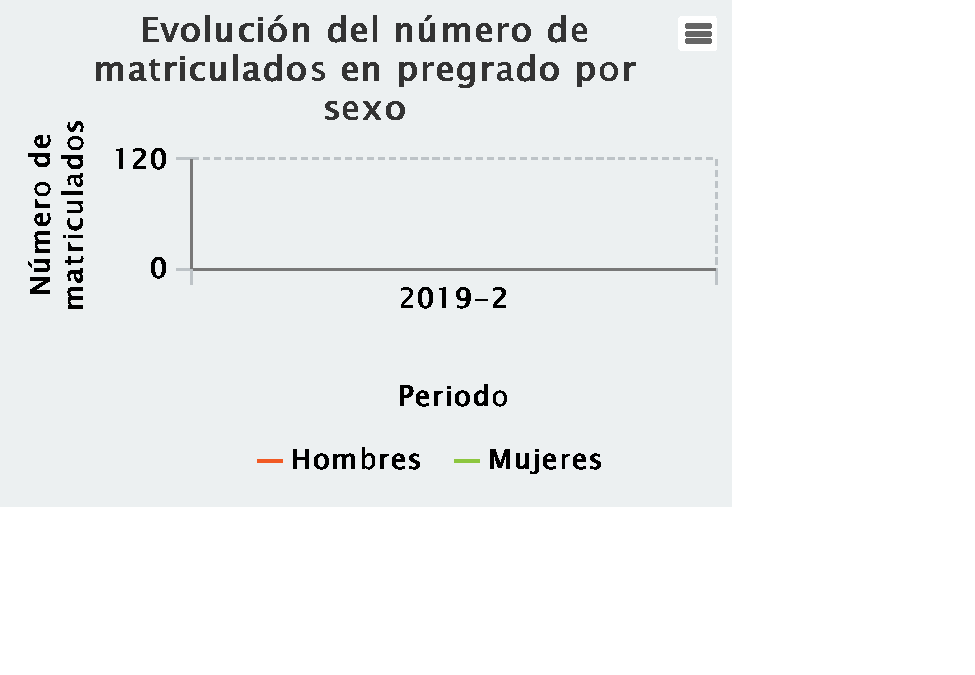
\includegraphics{BoletinLaPaz_files/figure-latex/F2MatPre-1.pdf}
\caption{\label{fig:F2MatPre}Fuente: Dirección Nacional de Planeación y Estadística con base en información de la Dirección Nacional Información Académica}
\end{figure}

\begin{figure}
\centering
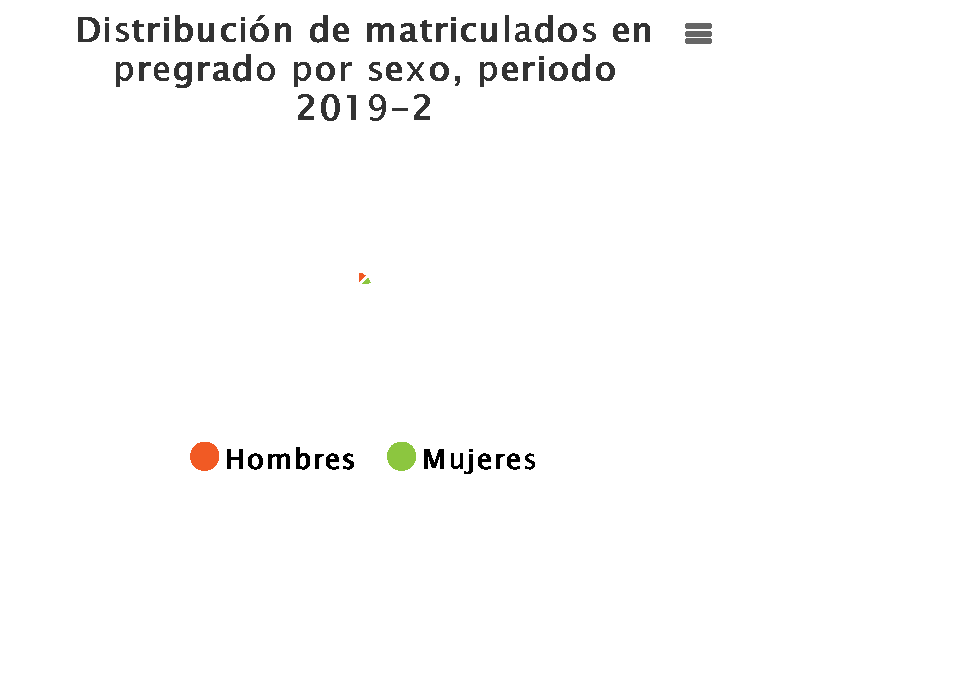
\includegraphics{BoletinLaPaz_files/figure-latex/F3MatPre-1.pdf}
\caption{\label{fig:F3MatPre}Fuente: Dirección Nacional de Planeación y Estadística con base en información de la Dirección Nacional Información Académica}
\end{figure}

\hypertarget{informaciuxf3n-por-edad-2}{%
\subsection{Información por edad}\label{informaciuxf3n-por-edad-2}}

A continuación, las figuras \ref{fig:F4MatPre} y \ref{fig:F5MatPre} presentan, respectivamente, la evolución histórica y el comportamiento actual del total de estudiantes matriculados en pregrado de la \textbf{Sede La Paz} según grupos de edad.

\begin{figure}
\centering
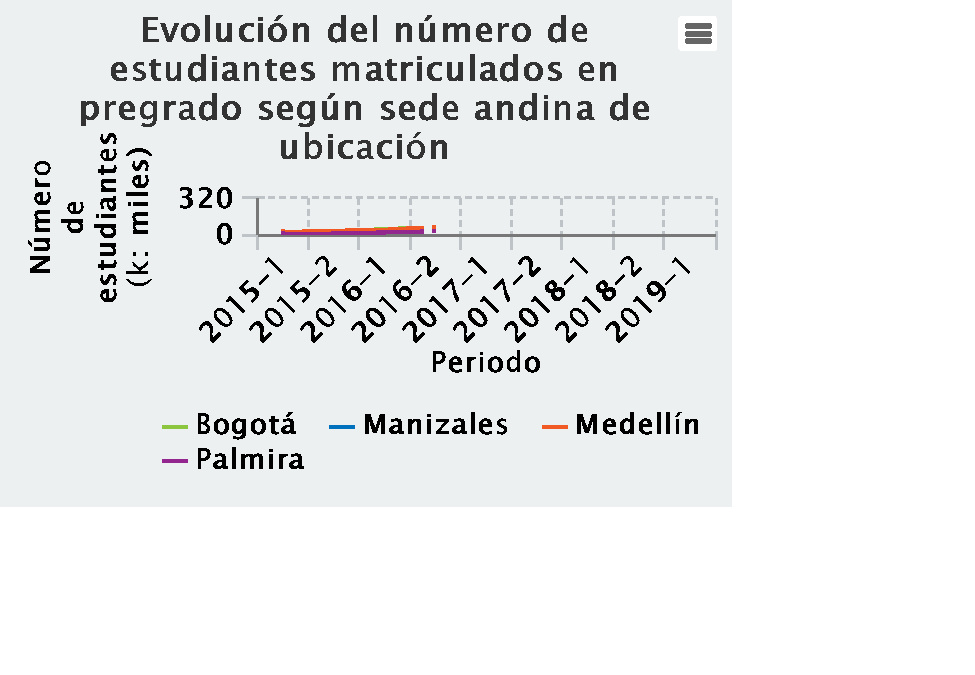
\includegraphics{BoletinLaPaz_files/figure-latex/F4MatPre-1.pdf}
\caption{\label{fig:F4MatPre}Fuente: Dirección Nacional de Planeación y Estadística con base en información de la Dirección Nacional Información Académica}
\end{figure}

\begin{figure}
\centering
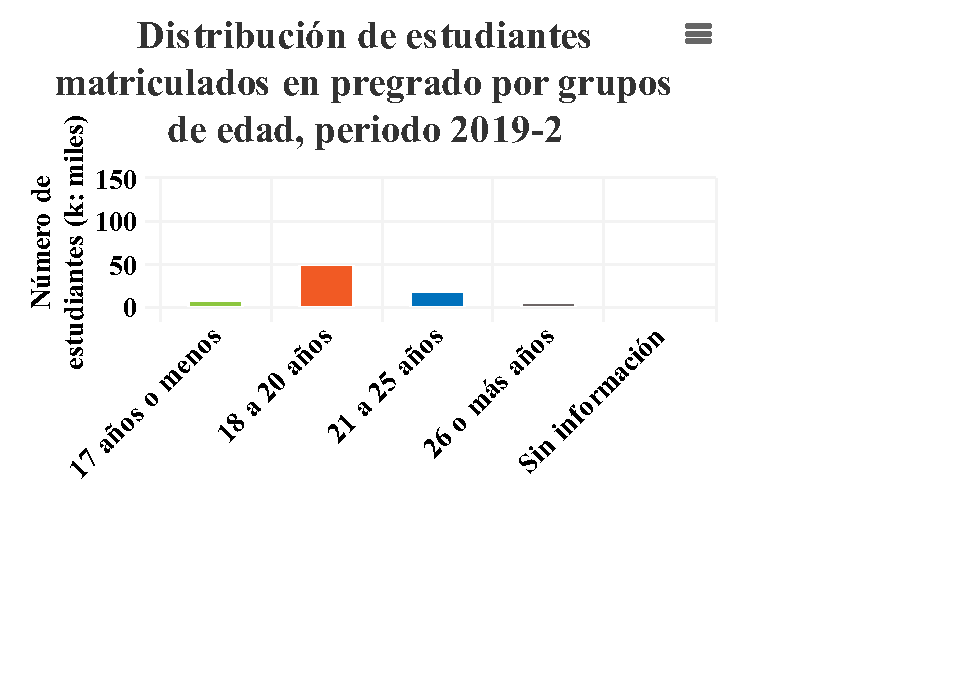
\includegraphics{BoletinLaPaz_files/figure-latex/F5MatPre-1.pdf}
\caption{\label{fig:F5MatPre}Fuente: Dirección Nacional de Planeación y Estadística con base en información de la Dirección Nacional Información Académica}
\end{figure}

\hypertarget{informaciuxf3n-por-estrato}{%
\subsection{Información por estrato}\label{informaciuxf3n-por-estrato}}

A continuación, las figuras \ref{fig:F6MatPre} y \ref{fig:F7MatPre} presentan, respectivamente, la evolución histórica y el comportamiento actual del total de estudiantes matriculados en pregrado en la \textbf{Sede La Paz} según el estrato socioeconómico.

\begin{figure}
\centering
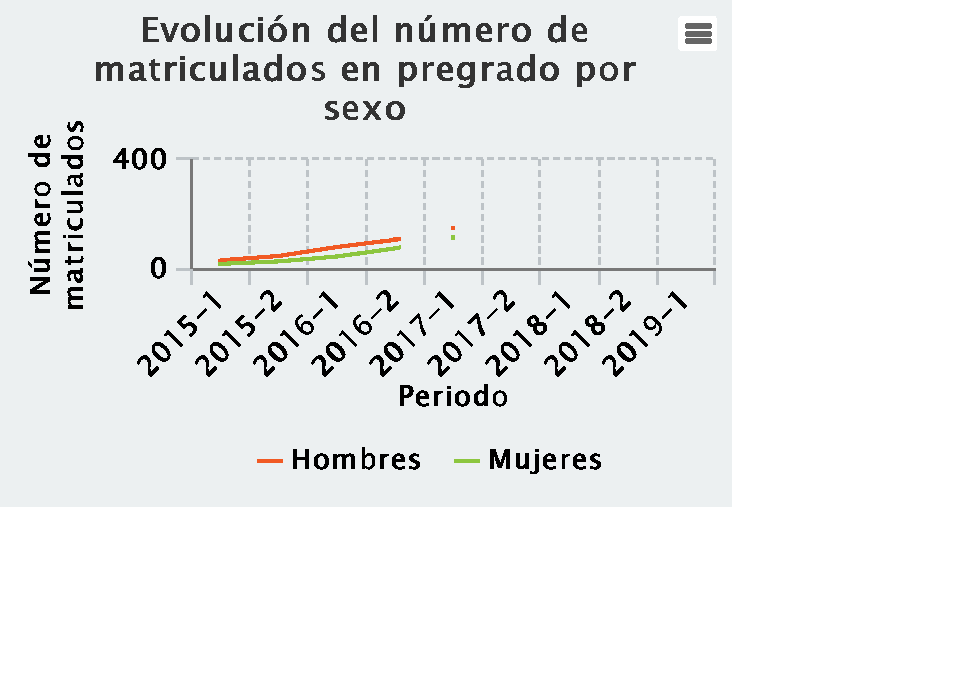
\includegraphics{BoletinLaPaz_files/figure-latex/F6MatPre-1.pdf}
\caption{\label{fig:F6MatPre}Fuente: Dirección Nacional de Planeación y Estadística con base en información de la Dirección Nacional Información Académica}
\end{figure}

\begin{figure}
\centering
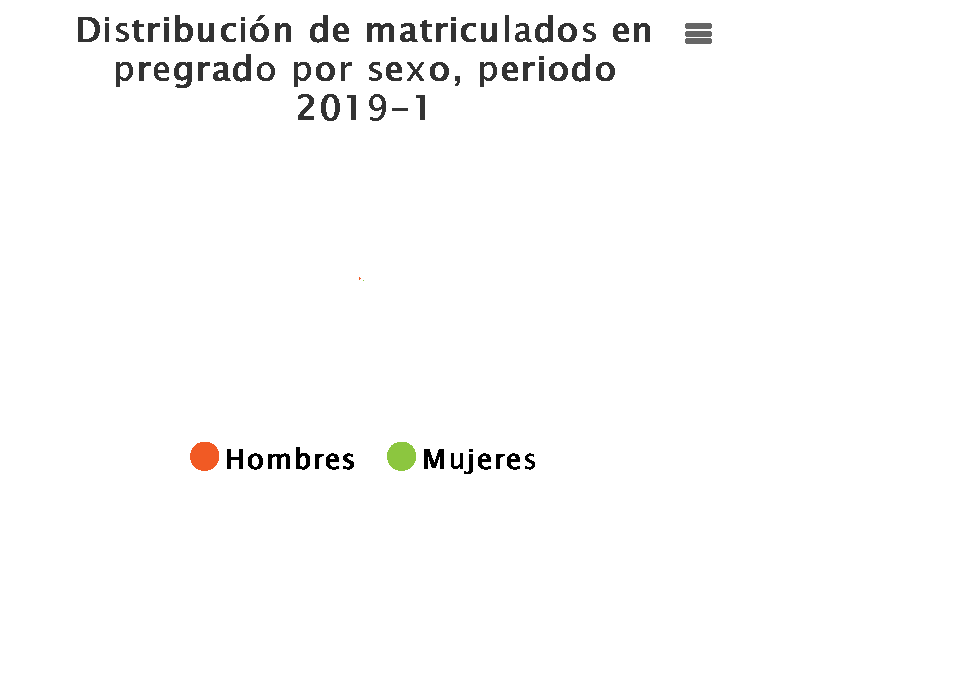
\includegraphics{BoletinLaPaz_files/figure-latex/F7MatPre-1.pdf}
\caption{\label{fig:F7MatPre}Fuente: Dirección Nacional de Planeación y Estadística con base en información de la Dirección Nacional Información Académica}
\end{figure}

\hypertarget{tablas-cifras-agregadas-2}{%
\subsection{Tablas cifras agregadas}\label{tablas-cifras-agregadas-2}}

A continuación se presentan, a través de tablas, los agregados/consolidados históricos del total de matriculados en pregrado de la \textbf{Sede La Paz} por departamentos y municipios de procedencia así como los programas académicos de pregrado que estos cursan en las sedes andinas de la Universidad (Bogotá, Medellín, Manizales y Palmira).

Los interesados en \emph{imprimir}, \emph{copiar} o \emph{descargar} estas cifras, pueden hacerlo a través de las múltiples opciones que se ofrecen en la parte superior izquierda de cada una de las tablas (Copiar, CSV, Excel, PDF e Imprimir). Así mismo, estas tablas permiten filtrar los resultados por aquellas variables de interés.

\hypertarget{departamentos-y-municipios-de-procedencia-1}{%
\subsubsection{Departamentos y municipios de procedencia}\label{departamentos-y-municipios-de-procedencia-1}}

A continuación, la Tabla \ref{fig:F8MatPre} presenta los acumulados \textbf{históricos}, por \textbf{años y semestres}, en la \textbf{Sede La Paz}, de los matriculados en pregrado por departamentos y municipios de procedencia.

\begin{figure}
\centering
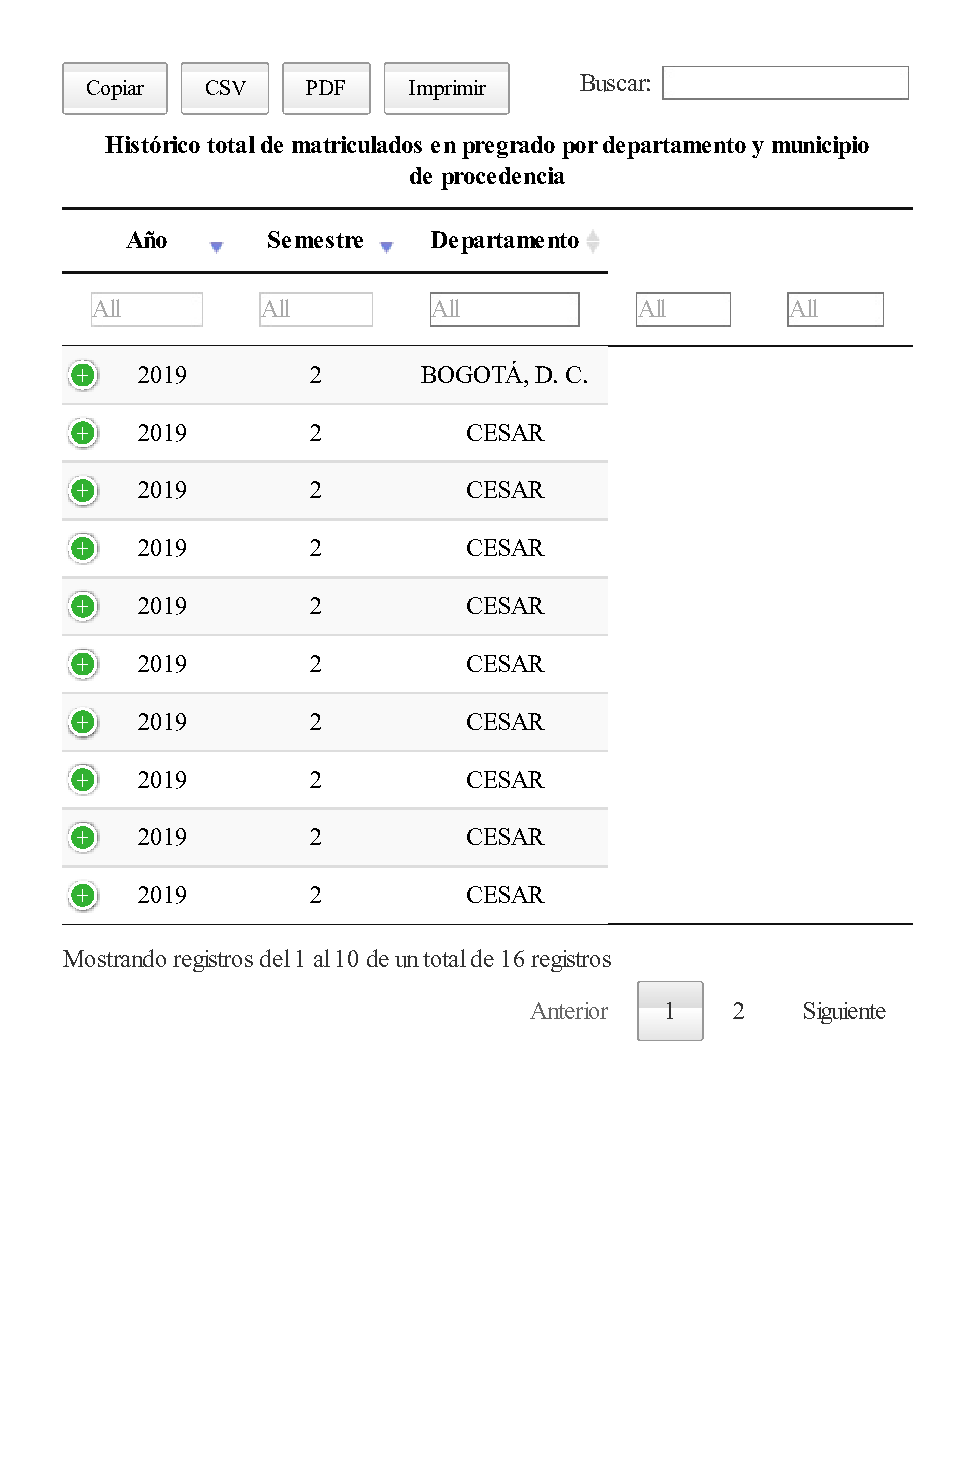
\includegraphics{BoletinLaPaz_files/figure-latex/F8MatPre-1.pdf}
\caption{\label{fig:F8MatPre}Fuente: Dirección Nacional de Planeación y Estadística con base en información de la Dirección Nacional Información Académica}
\end{figure}

\hypertarget{programas-acaduxe9micos-de-pregrado-1}{%
\subsubsection{Programas académicos de pregrado}\label{programas-acaduxe9micos-de-pregrado-1}}

A continuación, la Tabla \ref{fig:F9MatPre} presenta el acumulado histórico de matriculados en pregrado en la \textbf{Sede La Paz}, por años, semestres, sedes andinas, facultades y programas académicos cursados.

\begin{figure}
\centering
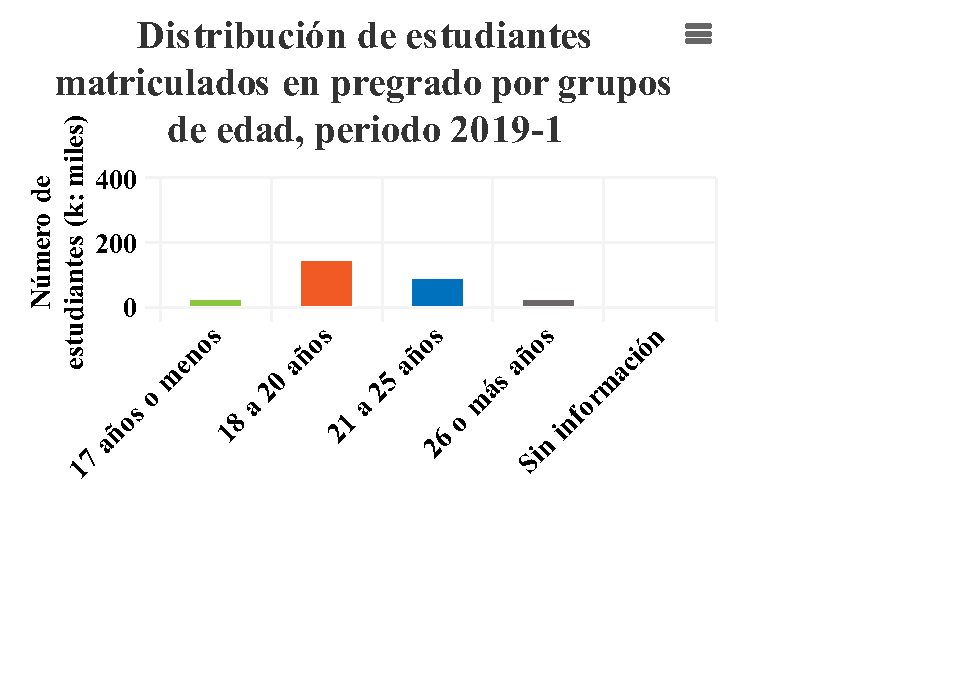
\includegraphics{BoletinLaPaz_files/figure-latex/F9MatPre-1.pdf}
\caption{\label{fig:F9MatPre}Fuente: Dirección Nacional de Planeación y Estadística con base en información de la Dirección Nacional Información Académica}
\end{figure}

\hypertarget{Grad}{%
\chapter{Graduados}\label{Grad}}

La \textbf{Sede La Paz} de la Universidad Nacional de Colombia, dada la \textbf{reciente apertura} para la formación de estudiantes en programas académicos de pregrado (2020-1), \textbf{aún no cuenta con estudiantes graduados en este nivel de formación}. Se espera que los primeros graduados de pregrado en esta sede de la Universidad se presenten entre los años 2024 y 2025.

\hypertarget{Doc}{%
\chapter{Docentes}\label{Doc}}

Este capítulo presenta el consolidado de las principales características asociadas a la información estadística oficial de los docentes de carrera adscritos a la Sede La Paz de la Universidad Nacional de Colombia.

A continuación, se presenta una breve descripción de las secciones que hacen parte de este capítulo así como la ubicación del sitio web en donde se presentan las definiciones, los estándares y las codificaciones/clasificaciones que hacen parte de la información acá contenida (\emph{metadatos}) y cuya exploración y lectura facilitará el entendimiento de las cifras asociadas a la población de docentes de carrera en esta sede de la Universidad.

\textbf{Secciones}

\begin{itemize}
\tightlist
\item
  \protect\hyperlink{DocCar}{Docentes de carrera}: contiene la información oficial del total de docentes de carrera adscritos a la Sede La Paz de la Universidad Nacional de Colombia y que fueron vinculados mediante concurso profesoral abierto y público o por reingreso a la carrera docente.
\end{itemize}

\textbf{Metadatos}

La construcción de las cifras oficiales de docentes de carrera en la Sede La Paz, las definiciones que hacen parte de esta categoría así como las codificaciones y clasificaciones aquí empleadas se encuentran contenidas en la sección \textbf{Docentes} del capítulo de \emph{Metadatos} de las cifras oficiales generales que hacen parte de la página de \href{http://estadisticas.unal.edu.co/home/}{estadísticas} de la Universidad Nacional de Colombia. Invitamos a los lectores a explorar y conocer estos metadatos los cuales, además de orientar y facilitar el entendimiento de la información de docentes de carrera, se encuentran disponibles en el siguiente enlace.

\begin{itemize}
\tightlist
\item
  \href{http://estadisticas.unal.edu.co/menu-principal/cifras-generales/metadatos/cifras-generales/}{Metadatos Cifras Oficiales Universidad Nacional de Colombia}
\end{itemize}

\hypertarget{DocCar}{%
\section{Docentes de carrera}\label{DocCar}}

A continuación, se presentan las principales características asociadas a los docentes de carrera de la \textbf{Sede La Paz} de la Universidad Nacional de Colombia. En específico, se presenta la evolución histórica de los docentes desde diferentes perspectivas: general, sexo, grupos de edad y máximo nivel de formación. Para cada una de las variables analizadas se presenta la evolución histórica (\emph{serie de tiempo}) así como el comportamiento actual (\emph{estado actual}) derivado de las últimas mediciones disponibles.

Nota: Número de docentes de carrera

El número de docentes de carrera en la Sede La Paz de la Universidad es bajo. Este hecho implica leer con precaución las frecuencias relativas (porcentajes) presentes en algunos de los resultados que se presentan a continuación. Estos, por por los bajos tamaños poblacionales existentes, son altamentente inestables/volátiles.

\hypertarget{evoluciuxf3n-histuxf3rica-3}{%
\subsection{Evolución Histórica}\label{evoluciuxf3n-histuxf3rica-3}}

A continuación, la Figura \ref{fig:F1DocCar}, presenta la evolución histórica -\emph{desde el periodo 20191}-, del total de docentes de carrera de la \textbf{Sede La Paz}.

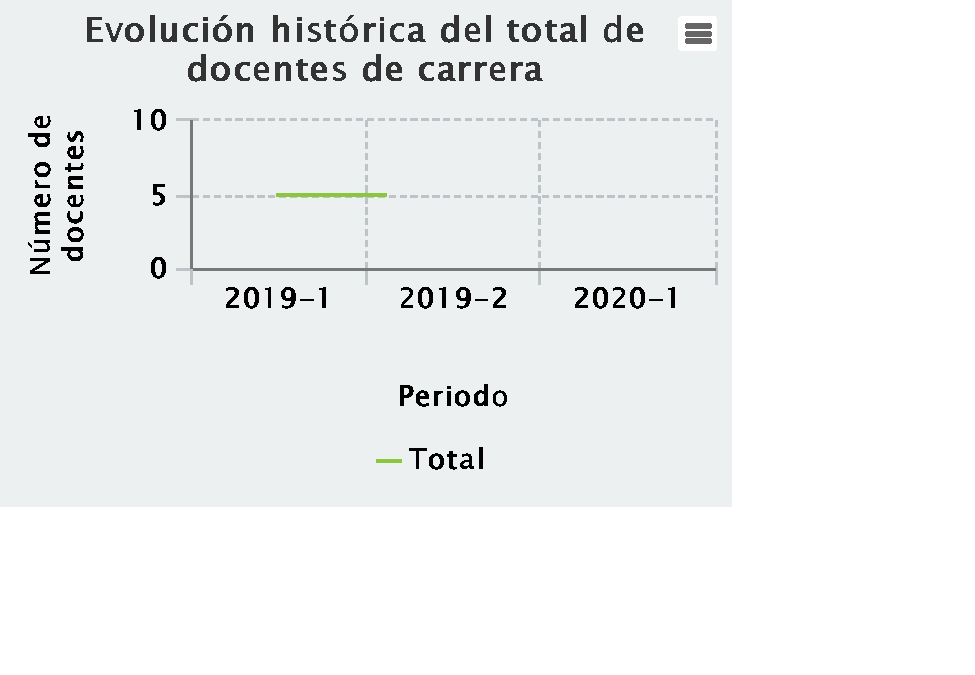
\includegraphics{BoletinLaPaz_files/figure-latex/F1DocCar-1.pdf}

\hypertarget{informaciuxf3n-por-sexo-3}{%
\subsection{Información por sexo}\label{informaciuxf3n-por-sexo-3}}

A continuación, las figuras \ref{fig:F2DocCar} y \ref{fig:F3DocCar} presentan, respectivamente, la evolución histórica y el comportamiento actual del total de docentes de carrera de la \textbf{Sede La Paz} según el sexo biológico.

\begin{figure}
\centering
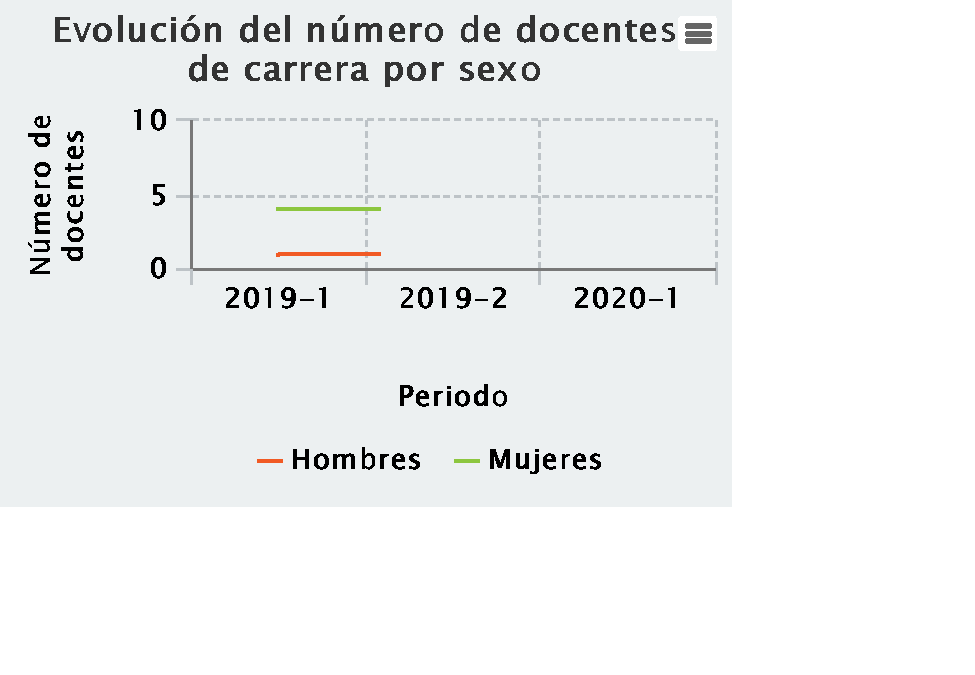
\includegraphics{BoletinLaPaz_files/figure-latex/F2DocCar-1.pdf}
\caption{\label{fig:F2DocCar}Fuente: Dirección Nacional de Planeación y Estadística con base en información de la Dirección Nacional de Talento Humano}
\end{figure}

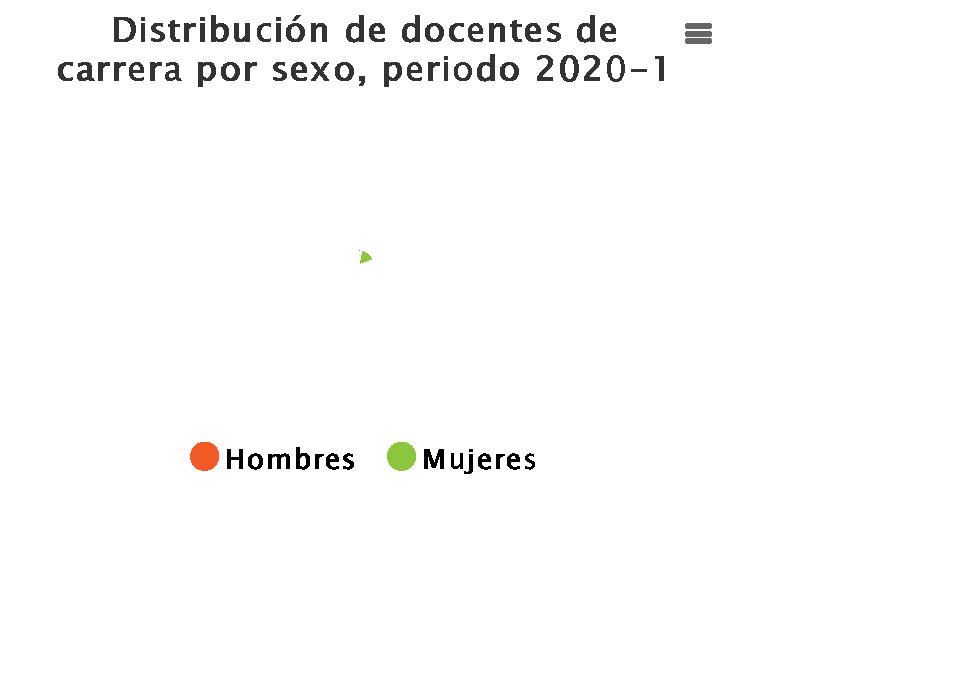
\includegraphics{BoletinLaPaz_files/figure-latex/F3DocCar-1.pdf}

\hypertarget{informaciuxf3n-por-edad-3}{%
\subsection{Información por edad}\label{informaciuxf3n-por-edad-3}}

A continuación, las figuras \ref{fig:F4DocCar} y \ref{fig:F5DocCar} presentan, respectivamente, la evolución histórica y el comportamiento actual del total de docentes de carrera de la \textbf{Sede La Paz} según grupos de edad.

\begin{figure}
\centering
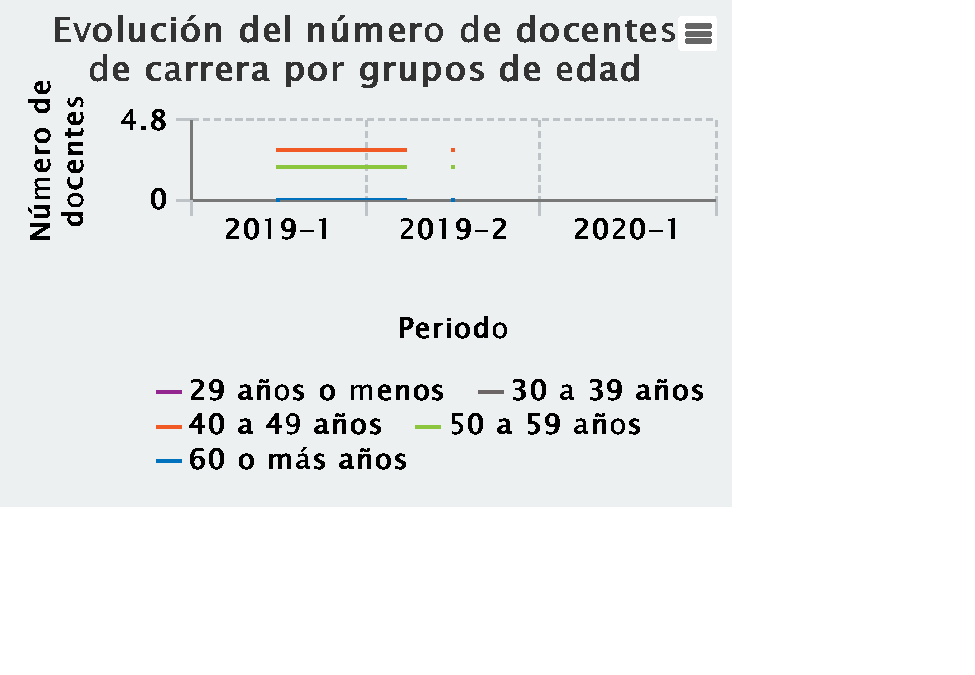
\includegraphics{BoletinLaPaz_files/figure-latex/F4DocCar-1.pdf}
\caption{\label{fig:F4DocCar}Fuente: Dirección Nacional de Planeación y Estadística con base en información de la Dirección Nacional de Talento Humano}
\end{figure}

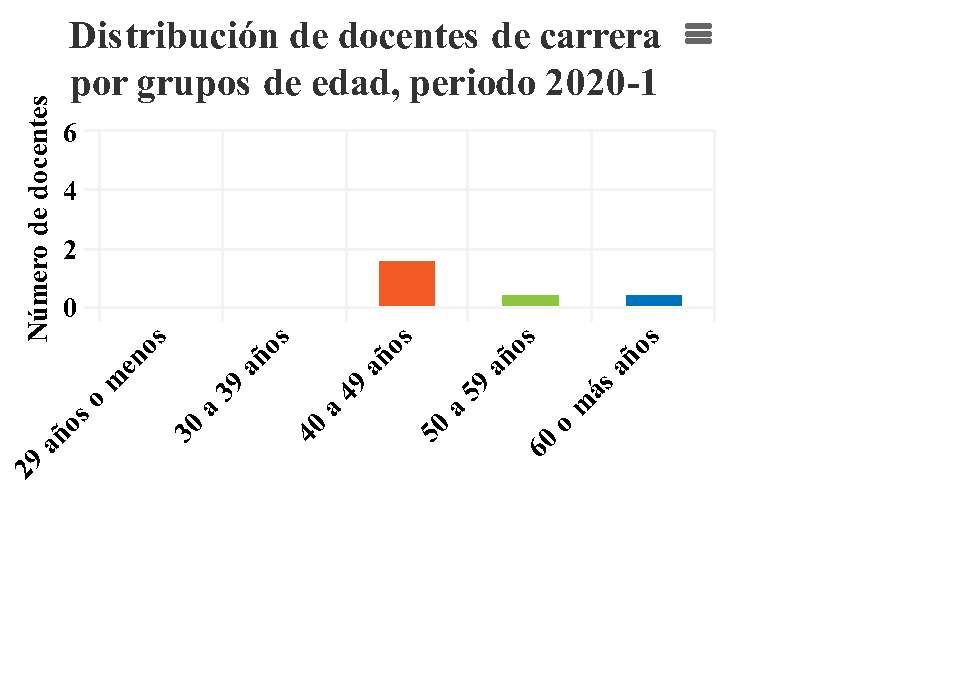
\includegraphics{BoletinLaPaz_files/figure-latex/F5DocCar-1.pdf}

\hypertarget{informaciuxf3n-por-muxe1ximo-nivel-de-formaciuxf3n}{%
\subsection{Información por máximo nivel de formación}\label{informaciuxf3n-por-muxe1ximo-nivel-de-formaciuxf3n}}

A continuación, las figuras \ref{fig:F6DocCar} y \ref{fig:F7DocCar} presentan, respectivamente, la evolución histórica y el comportamiento actual del total de docentes de carrera de la \textbf{Sede La Paz} según el máximo nivel de formación.

\begin{figure}
\centering
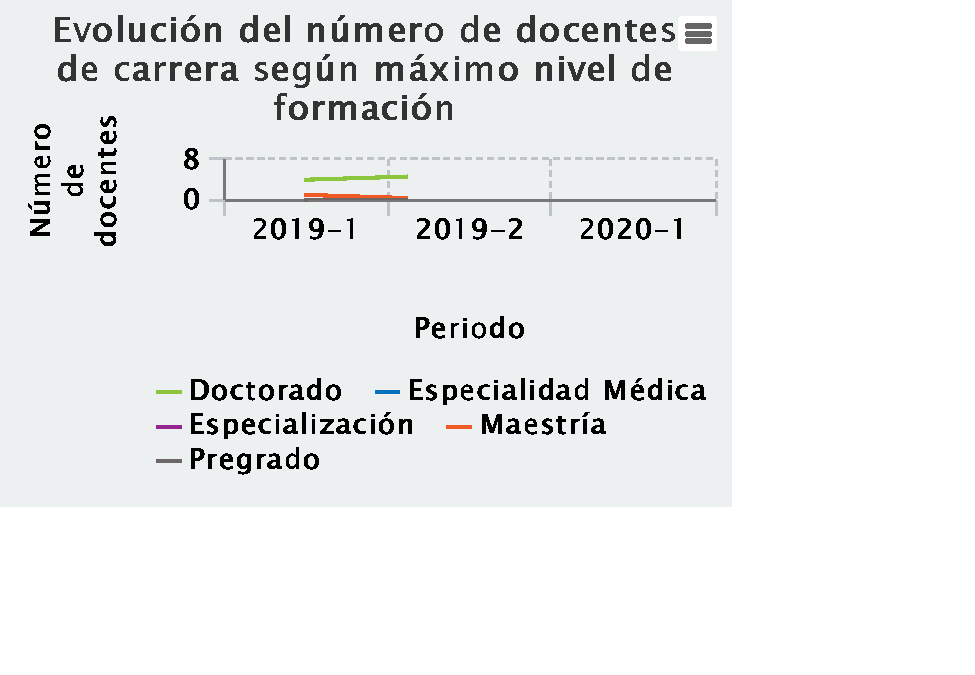
\includegraphics{BoletinLaPaz_files/figure-latex/F6DocCar-1.pdf}
\caption{\label{fig:F6DocCar}Fuente: Dirección Nacional de Planeación y Estadística con base en información de la Dirección Nacional de Talento Humano}
\end{figure}

\begin{figure}
\centering
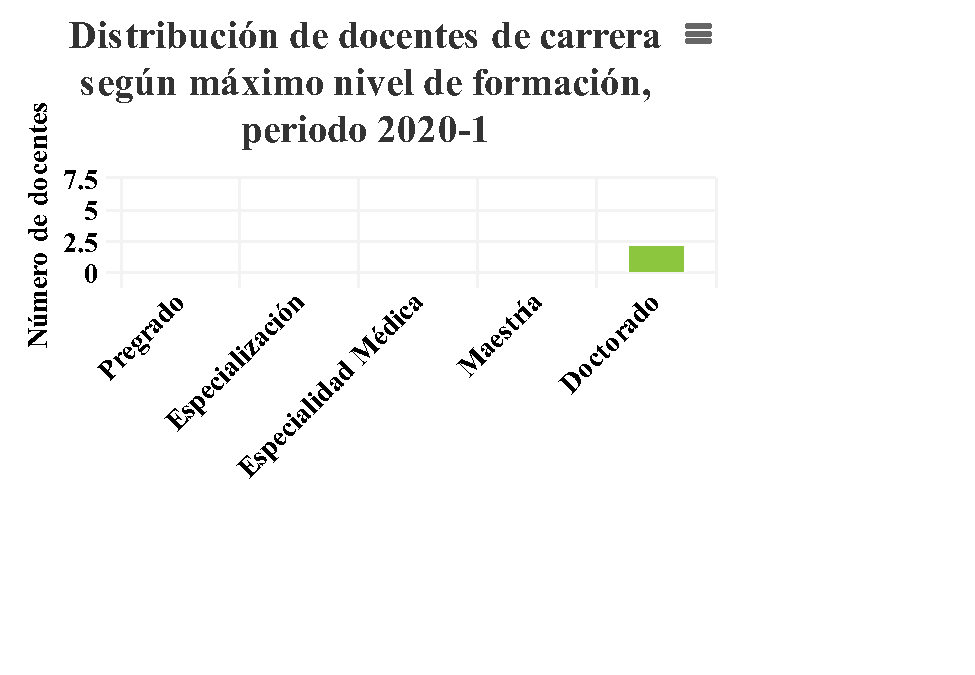
\includegraphics{BoletinLaPaz_files/figure-latex/F7DocCar-1.pdf}
\caption{\label{fig:F7DocCar}Fuente: Dirección Nacional de Planeación y Estadística con base en información de la Dirección Nacional de Talento Humano}
\end{figure}

\hypertarget{Admi}{%
\chapter{Administrativos}\label{Admi}}

Este capítulo presenta el consolidado de las principales características asociadas a la información estadística oficial de los administrativos de carrera adscritos a la Sede La Paz de la Universidad Nacional de Colombia.

A continuación, se presenta una breve descripción de las secciones que hacen parte de este capítulo así como la ubicación del sitio web en donde se presentan las definiciones, los estándares y las codificaciones/clasificaciones que hacen parte de la información acá contenida (\emph{metadatos}) y cuya exploración y lectura, sin duda, facilitará el entendimiento de las cifras asociadas a la población de administrativos de carrera en esta sede de la Universidad.

\textbf{Secciones}

\begin{itemize}
\tightlist
\item
  \protect\hyperlink{AdmCar}{Administrativos de carrera}: contiene la información oficial del total de funcionarios administrativos de carrera adscritos a la Sede La Paz de la Universidad Nacional de Colombia y que fueron vinculados mediante concurso público.
\end{itemize}

\textbf{Metadatos}

La construcción de las cifras oficiales de administrativos de carrera en la Sede La Paz, las definiciones que hacen parte de esta categoría así como las codificaciones y clasificaciones aquí empleadas se encuentran contenidas en la sección \textbf{Administrativos} del capítulo de \emph{Metadatos} de las cifras oficiales generales que hacen parte de la página de \href{http://estadisticas.unal.edu.co/home/}{estadísticas} de la Universidad Nacional de Colombia. Invitamos a los lectores a explorar y conocer estos metadatos los cuales, además de orientar y facilitar el entendimiento de la información de administrativos de carrera, se encuentran disponibles en el siguiente enlace.

\begin{itemize}
\tightlist
\item
  \href{http://estadisticas.unal.edu.co/menu-principal/cifras-generales/metadatos/cifras-generales/}{Metadatos Cifras Oficiales Universidad Nacional de Colombia}
\end{itemize}

\hypertarget{AdmCar}{%
\section{Administrativos de carrera}\label{AdmCar}}

A continuación, se presentan las principales características asociadas a los administrativos de carrera de la \textbf{Sede La Paz} de la Universidad Nacional de Colombia. En específico, se presenta la evolución histórica de los funcionarios administrativos desde diferentes perspectivas: general, sexo, grupos de edad y máximo nivel de formación. Para cada una de las variables analizadas se presenta la evolución histórica (\emph{serie de tiempo}) así como el comportamiento actual (\emph{estado actual}) derivado de las últimas mediciones disponibles.

Nota: Número de administrativos de carrera

El número de administrativos de carrera en la Sede La Paz de la Universidad es bajo. Este hecho implica leer con precaución las frecuencias relativas (porcentajes) presentes en algunos de los resultados que se presentan a continuación. Estos, por por los bajos tamaños poblacionales existentes, son altamentente inestables/volátiles.

\hypertarget{evoluciuxf3n-histuxf3rica-4}{%
\subsection{Evolución Histórica}\label{evoluciuxf3n-histuxf3rica-4}}

A continuación, la Figura \ref{fig:F1AdmiCar}, presenta la evolución histórica -\emph{desde el periodo 20191}-, del total de funcionarios administrativos de carrera de la \textbf{Sede La Paz}.

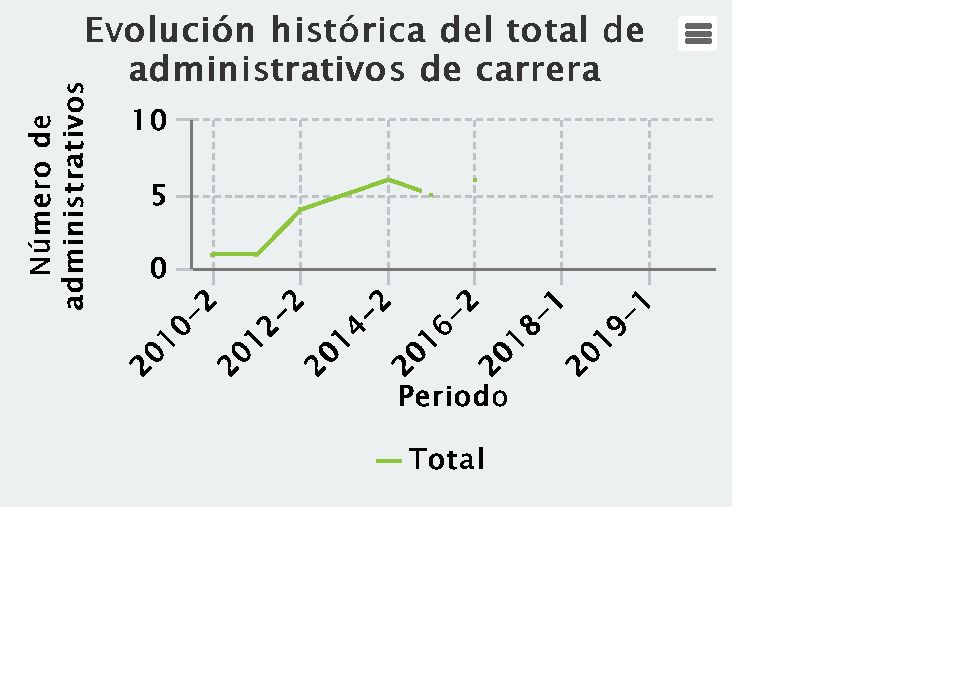
\includegraphics{BoletinLaPaz_files/figure-latex/F1AdmiCar-1.pdf}

\hypertarget{informaciuxf3n-por-sexo-4}{%
\subsection{Información por sexo}\label{informaciuxf3n-por-sexo-4}}

A continuación, las figuras \ref{fig:F2AdmiCar} y \ref{fig:F3AdmiCar} presentan, respectivamente, la evolución histórica y el comportamiento actual del total de funcionarios administrativos de carrera de la \textbf{Sede La Paz} según el sexo biológico.

\begin{figure}
\centering
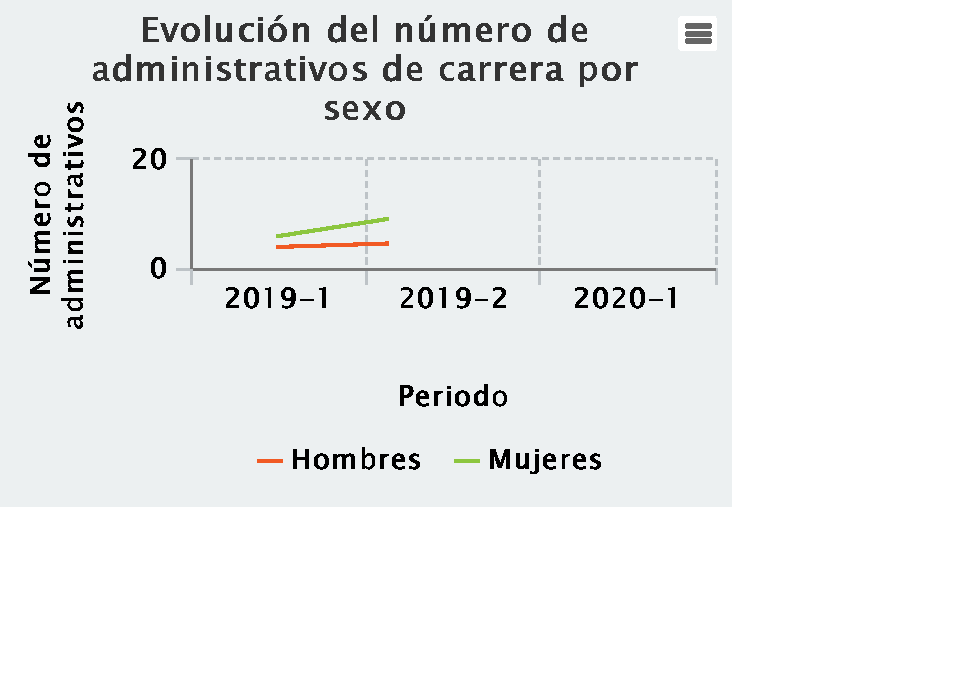
\includegraphics{BoletinLaPaz_files/figure-latex/F2AdmiCar-1.pdf}
\caption{\label{fig:F2AdmiCar}Fuente: Dirección Nacional de Planeación y Estadística con base en información de la Dirección Nacional de Talento Humano}
\end{figure}

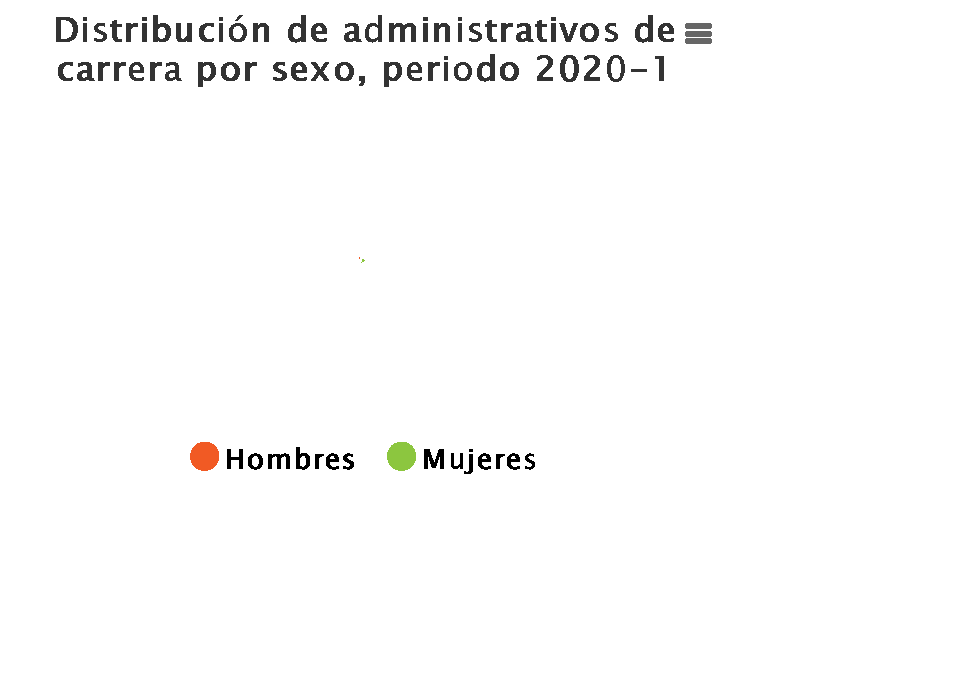
\includegraphics{BoletinLaPaz_files/figure-latex/F3AdmiCar-1.pdf}

\hypertarget{informaciuxf3n-por-edad-4}{%
\subsection{Información por edad}\label{informaciuxf3n-por-edad-4}}

A continuación, las figuras \ref{fig:F4AdmiCar} y \ref{fig:F5AdmiCar} presentan, respectivamente, la evolución histórica y el comportamiento actual del total de funcionarios administrativos de carrera de la \textbf{Sede La Paz} según grupos de edad.

\begin{figure}
\centering
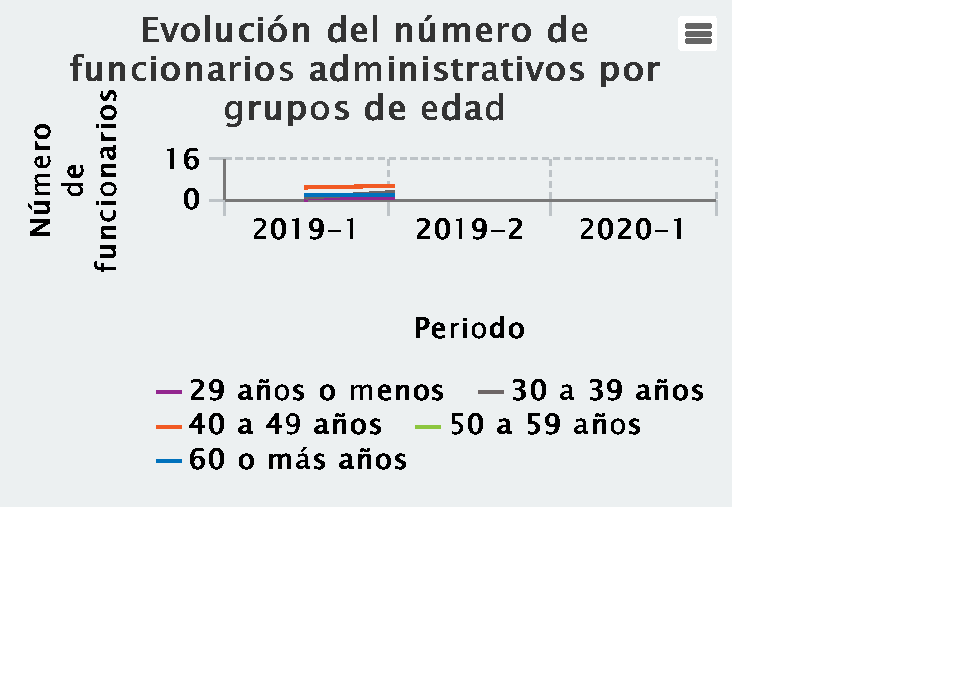
\includegraphics{BoletinLaPaz_files/figure-latex/F4AdmiCar-1.pdf}
\caption{\label{fig:F4AdmiCar}Fuente: Dirección Nacional de Planeación y Estadística con base en información de la Dirección Nacional de Talento Humano}
\end{figure}

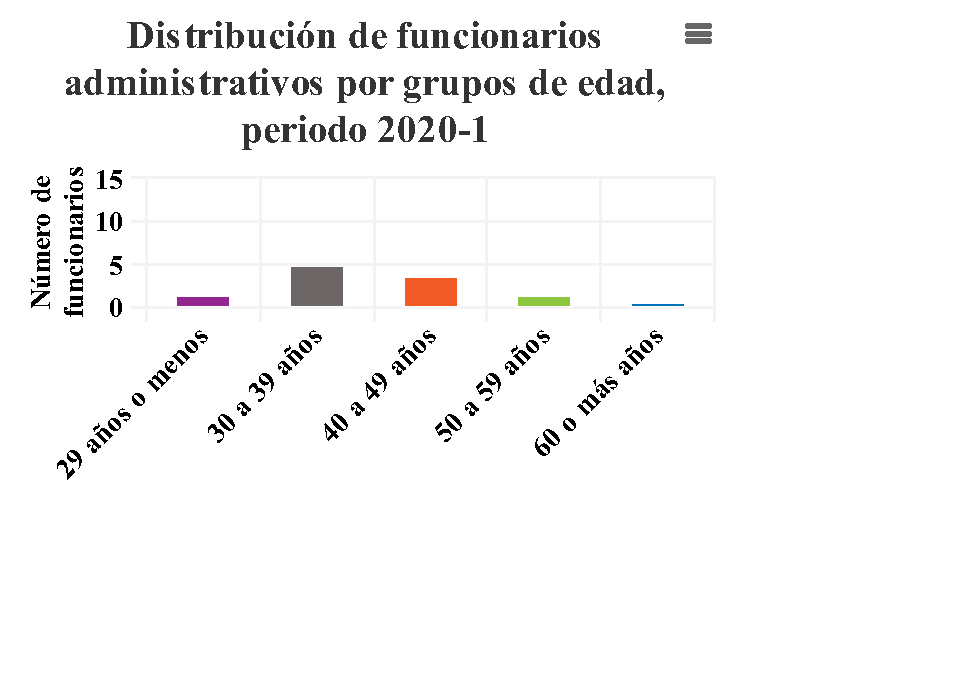
\includegraphics{BoletinLaPaz_files/figure-latex/F5AdmiCar-1.pdf}

\hypertarget{informaciuxf3n-por-muxe1ximo-nivel-de-formaciuxf3n-1}{%
\subsection{Información por máximo nivel de formación}\label{informaciuxf3n-por-muxe1ximo-nivel-de-formaciuxf3n-1}}

A continuación, las figuras \ref{fig:F6AdmiCar} y \ref{fig:F7AdmiCar} presentan, respectivamente, la evolución histórica y el comportamiento actual del total de funcionarios administrativos de carrera de la \textbf{Sede La Paz} según el máximo nivel de formación.

\begin{figure}
\centering
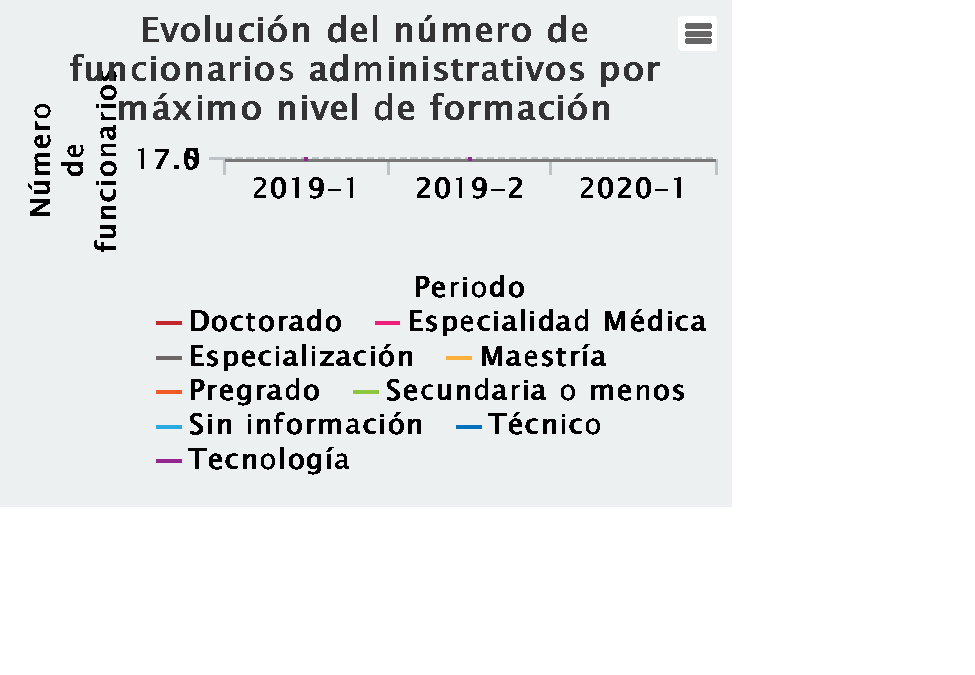
\includegraphics{BoletinLaPaz_files/figure-latex/F6AdmiCar-1.pdf}
\caption{\label{fig:F6AdmiCar}Fuente: Dirección Nacional de Planeación y Estadística con base en información de la Dirección Nacional de Talento Humano}
\end{figure}

\begin{figure}
\centering
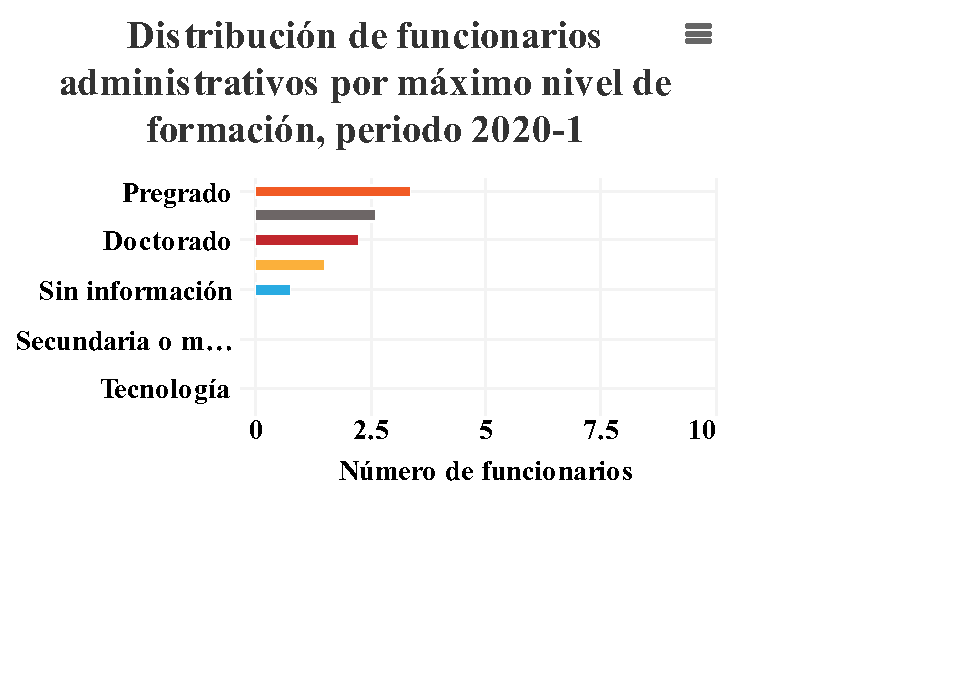
\includegraphics{BoletinLaPaz_files/figure-latex/F7AdmiCar-1.pdf}
\caption{\label{fig:F7AdmiCar}Fuente: Dirección Nacional de Planeación y Estadística con base en información de la Dirección Nacional de Talento Humano}
\end{figure}

\hypertarget{Inv}{%
\chapter{Investigación, Extensión e Innovación}\label{Inv}}

\hypertarget{investigaciuxf3n}{%
\section{Investigación}\label{investigaciuxf3n}}

\hypertarget{extensiuxf3n}{%
\section{Extensión}\label{extensiuxf3n}}

\hypertarget{Bie}{%
\chapter{Bienestar}\label{Bie}}

\hypertarget{gestiuxf3n-y-fomento-socioeconuxf3mico}{%
\section{Gestión y fomento socioeconómico}\label{gestiuxf3n-y-fomento-socioeconuxf3mico}}

  \bibliography{book.bib,packages.bib}

\end{document}
